\appendix
\chapter{Experimental Protocol and Reproducibility}\label{app:extended_results}

This appendix specifies the evaluation and reproduction protocols. Appendix~\ref{app:supp_experiments} contains the complete results, validation selections, ablations and qualitative examples.

\section{Split-Method Evaluation}

The campaigns retain the distinct attribution targets described in Section~\ref{sec:experimental_setup}. In the split campaign, misclassified images therefore pair the predicted-class attribution with another class's annotated mask.

\subsection{Artifact Availability and Reproduction Scope}\label{app:hm_artifact_scope}

The Hidden Monotonicity tables retain their published-source provenance. The code checkout lacks original per-image outputs, the complete historical evaluation environment, and six advertised MNIST multi-seed training configurations. The runnable notebook-derived example cannot reconstruct those missing settings, so the available artifacts cannot establish exact reproduction of the historical tables.

Deterministic CPU fixtures exercise double-precision reconstruction, input derivatives, attribution, timing, and Pixel Flipping with an independently evaluated initial target score. They establish the tested implementation contracts; agreement with the original ImageNet results remains unverified without a rerun. The historical training runner used the test loader for epoch validation. The current runner reserves a deterministic $10\%$ of training data for validation and evaluates the test set after training, recording partition indices and seed. This does not establish the checkpoint-selection procedure behind the historical MNIST figures.

\section{Evaluation Protocol}\label{ptnb:app:protocol}

\subsection{Data and splits}

The game-method campaign uses the released ImageNet-S50 validation annotations~\parencite{gao2022luss},
which contain $752$ images from $50$ classes. We exclude $136$ images whose annotation class
differs from the official ILSVRC2012 label, leaving $616$ eligible images. With seed $42$, one
image per class forms the \textbf{50-image validation split}, used only for configuration
selection; the remaining $566$ form the test pool. Images whose object mask lies entirely outside
the $224{\times}224$ center crop are excluded after the split, because the mask-based metrics are
undefined for them. This removes one test image and leaves \textbf{565 test images}. The
explanation target is the dataset class, including when the model misclassifies the image. This
population and target convention belong to the game-method protocol and need not coincide with
the split-method campaign. The Pascal VOC 2012 transfer split is described in
Section~\ref{ptnb:app:voc-cross-data}.

\subsection{Metric definitions}\label{ptnb:app:metrics}\label{app:metrics}

Let $x \in \RR^{C \times H \times W}$ be an image, let $y$ be its target class, and let $a \in
    \RR^{H \times W}$ be the scalar attribution map produced by an explanation method after channel
reduction. Write $d \coloneqq HW$ and let $\text{vec}(a) \in \RR^d$ denote the flattened map. For
any binary segmentation mask $m \in \{0,1\}^{H \times W}$, write $\text{vec}(m) \in \{0,1\}^d$.
When a metric is configured with \texttt{abs=true} and \texttt{normalise=true}, the evaluator
applies the max-abs normalization (not min--max)
\begin{align}
    \psi(a) = \frac{|\text{vec}(a)|}{\max_i |\text{vec}(a)_i|},
\end{align}
with the convention that the all-zero map remains zero. We denote the preprocessed attribution
vector by $\bar{a}$. All metrics below use $\bar{a}$; faithfulness metrics use raw logits (no
softmax) to avoid saturation effects, and perturbations use the Quantus per-sample mean replacement
baseline.

\paragraph{Attribution localization (AL).} We adapt \textcite{Kohlbrenner2020}'s positive-relevance ratio within ground-truth boxes to absolute mass, pixel masks, and a stabilized denominator:
\begin{align}
    \text{AL}(a, m) = \frac{\sum_{i=1}^d \bar{a}_i m_i}{\sum_{i=1}^d \bar{a}_i + 10^{-9}}.
\end{align}

\paragraph{Pointing game (PG).} We use the pointing-game criterion of~\textcite{Zhang2018pointinggame}; our configuration applies \texttt{abs=true} without normalization. Let $M(a) \coloneqq \{i \in \{1, \dots, d\} :
    \bar{a}_i = \max_j \bar{a}_j\}$ contain all maximizers. Then
\begin{align}
    \text{PG}(a, m) = \1\bigl\{M(a) \cap \{i : m_i = 1\} \neq \varnothing\bigr\}.
\end{align}
A tie scores a hit if any maximizer lies inside the mask. PG is binary per image--class record; its ImageNet-S test mean is a multiple of $1/565$.

\paragraph{Top-$k$ intersection (TK).} Following~\textcite{Theiner2021}, with $k = 1000$ and the permutation $\pi$ that sorts
$\bar{a}$ in descending order:
\begin{align}
    \text{TK}(a, m) = \frac{1}{1000} \sum_{r=1}^{1000} m_{\pi_r}.
\end{align}

\paragraph{Pixel-flipping AUC (PF$_5$, PF$_{20}$).} Pixel flipping~\parencite{Bach2015,Samek2017evaluating} removes the most relevant features first
and tracks the class score. The evaluator uses \texttt{pixel\_flipping\_abs} with
\texttt{features\_in\_step = 1568} and \texttt{perturb\_baseline = mean}. Unlike the spatial
localization metrics above, pixel flipping operates on $D \coloneqq CHW$ scalar input features.
The spatial attribution is broadcast over the color channels; let $\widetilde\pi$ sort the
flattened broadcast attribution in descending order. For $T \coloneqq \lceil D/1568 \rceil$, the
input $x^{(t)}$ is obtained from $x^{(t-1)}$, starting at $x^{(0)}=x$, by replacing features
$\widetilde\pi_{(t-1)\cdot1568+1},\dots,\widetilde\pi_{\min\{t\cdot1568,D\}}$ with the scalar mean
of the current flattened input, as implemented by Quantus.
The evaluator computes
\begin{align}
    f_t \coloneqq F(x^{(t)})_y, \qquad t = 1, \dots, T,
\end{align}
and PF$_p$ is the trapezoidal area over the first $p\%$ of this flipping curve, i.e.\ over its
first $K_p$ points with the abscissa rescaled to $[0,1]$: $\text{PF}_p =
    \text{trapz}\bigl(\{(t-1)/(K_p-1), f_t\}_{t=1}^{K_p}\bigr)$, $K_p = \max(2, \lceil pT/100 \rceil)$.
For $C=3$ and $H=W=224$, $D=150{,}528$ and $T=96$ steps, giving $K_5=5$ and $K_{20}=20$.
The curve contains only post-perturbation scores; the original input score is not an additional
point. Lower is better.

\paragraph{Selectivity (Sel).} Following~\textcite{Montavon2018} and Quantus~\parencite{Hedstrom2023}, sum $\bar{a}$ over square $39{\times}39$ patches (side $\lfloor\sqrt{1568}\rfloor$). Replace non-overlapping patches by the per-sample mean in decreasing attribution order, recording the target logit after each removal. Sel is the trapezoidal area under this curve against the fraction of removed patches. Lower is better.

\paragraph{Max and average sensitivity (MaxS, AvgS).} Following~\textcite{Yeh2019}'s max-sensitivity and its mean analogue, regenerate attributions for both metrics on the same $N_s = 50$ inputs $x + \xi_k$, with uniform noise $\xi_k \sim \mathcal{U}[-r, r]^{C \times H
    \times W}$, $r = 0.2$. Report the maximum (MaxS) or mean (AvgS) over $k$ of $\|\psi(a(x+\xi_k)) - \psi(a(x))\|_F / \|\psi(a(x))\|_F$; lower values indicate greater stability to input noise. Per-image seeds give every row identical perturbations. Both metrics use the same fixed random subset of 200 test images (seed 0) across rows and models; all other metrics use the full test split.

\subsection{Selection}\label{ptnb:app:selection}

Every tunable method, including baselines, selects two configurations on validation: \texttt{loc} minimizes rank-sum over $\{\text{AL}, \text{PG}, \text{TK}\}$, and \texttt{faith} over $\{\text{PF}_5, \text{PF}_{20}, \text{Sel}\}$. Ranks are within-method and respect metric directions. Ties favor the default (the anchor for \ac{rg}), then fewer non-default parameters, then grid order. Admission requires non-zero maps and defined metrics on every validation image. Before ranking, we exclude 5 of the 40 VGG-16 \ac{sg} configurations, all with strong risk aversion and deterministic gates, whose maps vanish on some images; all others qualify. MaxS and AvgS are excluded from selection because each evaluation re-explains every image $2N_s$ times. The main discussion uses \texttt{loc}; Section~\ref{ptnb:app:results} reports both selections. Localization suits modes controlling routing focus, has external mask ground truth, and has precedent for comparing \ac{lrp} rules using bounding boxes~\parencite{Kohlbrenner2020}. Perturbation metrics evaluate off-distribution inputs. Reporting both selections preserves the distinction and trade-off between localization and faithfulness.

\subsection{Statistics}\label{ptnb:app:stats}

The game-method test tables report 95\% percentile bootstrap confidence
intervals~\parencite{Efron1993bootstrap} using $B=10{,}000$ resamples and seed~$0$. On ImageNet-S,
the sampling units are images, with the same resampled image indices used across method rows.
MaxS and AvgS intervals resample the fixed 200-image subset of Section~\ref{ptnb:app:metrics}.
Continuous metrics use a two-sided paired bootstrap test of the mean per-image difference: the
bootstrap distribution is centered at zero, and $p$ is the fraction of centered resampled
differences at least as large in absolute value as the observed difference. Binary PG uses
McNemar's test~\parencite{McNemar1947} with continuity correction.

On Pascal VOC, the estimand remains the mean over image--class records, but the independent
sampling units are the $G=2{,}293$ original test images. Each bootstrap replicate samples $G$
images with replacement and retains every class record of each sampled image. Its mean is the sum
over these records divided by their replicate-specific count. Thus, classes from the same image
remain together, while images with more evaluated classes retain their contribution to the
reported record-weighted mean. Paired comparisons use common finite records and common image
draws. Every VOC metric, including binary PG, uses the corresponding two-sided, null-centered
paired cluster-bootstrap test. For observed mean difference $\widehat\Delta$ and bootstrap
differences $\Delta_b^*$, its finite-resample $p$-value is
\begin{align}
    p=\frac{1+\sum_{b=1}^{B}\1\{\lvert\Delta_b^*-\widehat\Delta\rvert
        \geq\lvert\widehat\Delta\rvert\}}{B+1}.
\end{align}

For the original localization-selected comparison and the full test tables, Holm correction~\parencite{Holm1979} is applied to all unordered
pairs of eligible rows within each metric and reported table, before extracting comparisons with
the observed best row or declaring a row ahead of every baseline. The observed winner therefore
does not determine the comparison family. A difference is called significant at adjusted
$p<0.05$; otherwise, no difference was detected at this threshold. This does not establish
practical equivalence. These intervals and tests condition on the fixed checkpoints, selected
configurations and realized attribution evaluations; they do not quantify training or
configuration-selection variability. The split-method tables report the source point estimates
without corresponding confidence intervals.

\section{Implementation and Evaluation Details}\label{app:extended_protocol}

\paragraph{Backbone and dataset provenance.}
All game-based experiments use the pretrained checkpoints shipped with the evaluation release of torchvision: VGG-16 uses \path{VGG16_Weights.IMAGENET1K_V1}
(\url{https://download.pytorch.org/models/vgg16-397923af.pth}; recipe
\url{https://github.com/pytorch/vision/tree/main/references/classification#alexnet-and-vgg}),
ResNet-50 uses \path{ResNet50_Weights.IMAGENET1K_V2}
(\url{https://download.pytorch.org/models/resnet50-11ad3fa6.pth}; recipe
\url{https://github.com/pytorch/vision/issues/3995#issuecomment-1013906621}), and ViT-B/16 uses
\path{ViT_B_16_Weights.IMAGENET1K_V1}
(\url{https://download.pytorch.org/models/vit_b_16-c867db91.pth}; recipe
\url{https://github.com/pytorch/vision/tree/main/references/classification#vit_b_16}). These ImageNet-1K classifiers were trained on ImageNet / ILSVRC~\parencite{Deng2009,Russakovsky2015ilsvrc} and scored with Quantus~\parencite{Hedstrom2023}.

\paragraph{Licenses.}\label{ptnb:app:licences}
ImageNet images~\parencite{Deng2009} are used under the ImageNet terms of access (non-commercial research and
educational use)\footnote{\url{https://www.image-net.org/download-images.php}.}. The ImageNet-S mask release~\parencite{gao2022luss} does not state a separate mask license\footnote{Authors' release: \url{https://github.com/LUSSeg/ImageNet-S}.}; its images are ImageNet images and fall under the same
terms. The Pascal VOC 2012 images are subject to the Flickr terms of use,
as stated by the dataset providers\footnote{\url{https://www.robots.ox.ac.uk/~vgg/projects/pascal/VOC/voc2012/}, Database Rights.}. The checkpoints are distributed with torchvision
and were trained on ImageNet-1K. Libraries: PyTorch and torchvision (BSD-3-Clause), Quantus
(GPL-3.0), zennit (GPL-3.0/LGPL-3.0), lxt, captum and scikit-image (BSD-3-Clause), pytorch-grad-cam
(MIT); the reference code of \acs{ptnbTIBAV} and \acs{ptnbGAE} (MIT) is included with its license notice.

\subsection{Methods}\label{ptnb:app:baselines}\label{app:baselines}

Baselines use lxt, zennit, captum, pytorch-grad-cam, and the authors' TIBAV/GAE code, with reference settings and the declared grids~\parencite{Achtibat2024AttnLRP,Anders2021Zennit,kokhlikyan2020captum,Gildenblat2021gradcam,Chefer2021GenericAttention,Chefer2021ICCV}.

\paragraph{Gradient-based block.}
\textbf{Gradient} is raw input-gradient saliency~\parencite{Simonyan2014}: the maximum absolute gradient over color channels. \textbf{SmGrad} averages noisy gradient maps (SmoothGrad)~\parencite{Smilkov2017}. \textbf{IntGrad} uses Integrated Gradients~\parencite{Sundararajan2017} with a black-image baseline. \textbf{DeepLIFT} propagates activation differences from a reference input using the Rescale rule~\parencite{Shrikumar2017} (CNNs only). \textbf{DAVE} is the distribution-aware ViT gradient decomposition of \textcite{Wrobel2024}; our implementation additionally freezes the LayerNorm mean, whereas published DAVE differentiates through mean-centering. \textbf{SG}, our \ac{sg}, belongs here because its occupation measure recovers the gradient (Theorem~\ref{ptnb:thm:deriv-occ}).

\paragraph{LRP / relevance-propagation block.}
\textbf{LRP-$\varepsilon$} is stabilized Layer-wise Relevance Propagation~\parencite{Bach2015}; \textbf{LRP-$\gamma$} amplifies positive weights~\parencite{Montavon_2022_gammaLRP}. \textbf{AttnLRP} propagates transformer relevance through softmax, the bilinear attention product and the Value path~\parencite{Achtibat2024AttnLRP}. \textbf{RG} is our \ac{rg}; \textbf{RG+Eq} adds equivariant Reynolds averaging, mainly to suppress ViT tokenization-grid artifacts. \textbf{TIBAV}~\parencite{Chefer2021GenericAttention}, \textbf{GAE}~\parencite{Chefer2021ICCV} and Attention Rollout (\textbf{AR}) are transformer attention-map baselines.

\paragraph{CAM block.}
\textbf{GCAM}, \textbf{GCAM++} and \textbf{LCAM} denote Grad-CAM~\parencite{Selvaraju2017}, Grad-CAM++~\parencite{Chattopadhay2018} and LayerCAM~\parencite{Jiang2021LayerCAM}, respectively. LayerCAM weights class-activation evidence per location. All three use the CNNs' last convolutional block and bilinear upsampling.

\paragraph{Perturbation block.}
\textbf{LIME} is Local Interpretable Model-agnostic Explanations~\parencite{Ribeiro2016}; \textbf{KernelSHAP} estimates SHAP values by model-agnostic weighted regression~\parencite{LundbergLee2017}. Both perturb SLIC superpixels~\parencite{Achanta2012slic} and fit local surrogates, distinguishing them from the backward-propagation methods.

\subsection{Declared validation grids}\label{ptnb:app:grids}

Table~\ref{ptnb:tab:main-search-grid} lists every method's grid. Functionally duplicate rows (e.g.\ different $\sigma^2$ when $\lambda = \lambda_{\mathrm{sm}} = 0$) are evaluated once, yielding \nValGrid{} configurations. On ViT-B/16, activation-side $\lambda$ is fixed to $0$, keeping GELU gates conditioned (Section~\ref{ptnb:sec:attention}). At attention--Value products, \ac{rg} applies $\alpha\beta$-\ac{lrp}-$\varepsilon$ to the composite attention-product/Value-projection map (Theorem~\ref{ptnb:thm:attn-ab-recovery}; Section~\ref{ptnb:app:vit-implementation}). Baselines without grids use their reference implementations' settings.

\begin{table}[H]
    \centering
    \caption[Per-method validation grids]{Per-method validation grids (all architectures unless stated). Symbols:
    Section~\ref{ptnb:app:config-symbols}.}
    \label{ptnb:tab:main-search-grid}
\TableContent{
    \small
    \renewcommand{\arraystretch}{1.15}
    \begin{tabularx}{\linewidth}{@{}l >{\raggedright\arraybackslash}X@{}}
        \toprule
        Method & Grid \\
        \midrule
        Gradient & single config \\
        SmGrad & $N{=}50$, noise level $\sigma/(x_{\max}{-}x_{\min}) \in \{0.1, 0.15, 0.2\}$, mean
        aggregation \quad (3 configs) \\
        IntGrad & black-image baseline, $N_{\text{steps}} \in \{20, 50, 100, 300\}$ \quad (4 configs) \\
        DeepLIFT & Rescale rule, single config \quad (CNNs only) \\
        DAVE & $N \in \{25, 50\} \times \theta_{\max} \in \{0, 10, 20\} \times s_{\max} \in \{0, 0.05,
            0.1\} \times t_{\max} \in \{0, 0.25, 0.5\}$, horizontal flips with probability $0.5$, averaged
        effective map multiplied by the input \quad (54 configs; ViT-B/16 only) \\
        SG & $\lambda \in \{-5, -2, -1, -0.3, 0\} \times \sigma^2 \in \{1, 2, 5, 10\} \times$ noisy gate
        $\tilde\Phi \in \{\text{off}, \text{on}\}$ \quad (40 configs; VGG-16 only) \\
        LRP-$\varepsilon$ & $\varepsilon \in \{0.01, 0.05, 0.1, 0.25, 0.5, 1, 2\}$ \quad (7 configs) \\
        LRP-$\gamma$ & $(\varepsilon, \gamma) \in \{0.1, 0.25, 0.5\}\times\{0.1, 0.25, 0.5, 1, 2\}$;
        ViT-B/16: $\gamma$ on all Linear layers (15 configs); CNNs: both zennit's EpsilonGammaBox composite
        ($z^{\mathcal{B}}$ input layer, $\gamma$ on convolutions, $\varepsilon$ on dense layers) and
        $\gamma$ on all layers (30 configs) \\
        AttnLRP & $\gamma$-composite of~\textcite{Achtibat2024AttnLRP}: reference setting
        $(\gamma_{\text{conv}}, \gamma_{\text{lin}}, \varepsilon_{\text{attn}}){=}(0.25, 0.05, 10^{-6})$ +
        univariate sweeps $\gamma_{\text{lin}}\in\{0.01, 0.025, 0.1, 0.25\}$,
        $\gamma_{\text{conv}}\in\{0.1, 0.5, 1\}$, $\varepsilon_{\text{attn}}\in\{0.01, 0.05,
            0.25\}$ \quad (11 configs; ViT-B/16 only) \\
        TIBAV & single config \quad (ViT-B/16 only) \\
        GAE & single config \quad (ViT-B/16 only) \\
        AR & residual weight $w_r \in \{0, 0.25, 0.5, 0.75\}$ \quad (4 configs; ViT-B/16 only) \\
        RG & $\tau \in \{0.3, 0.4, \ldots, 1.0\}$, $(\alpha,\beta){=}(2,1)$, $\sigma^2 \in \{1, 2, 5,
            10\}$, $\varepsilon \in \{0.1, 0.25, 0.5, 1\}$; ViT-B/16: $\lambda{=}0$, $\lambda_{\mathrm{sm}} \in
            \{-50, -10, -5, -2, -1, 0\}$, composite Value rule of Theorem~\ref{ptnb:thm:attn-ab-recovery} (672
        configs); CNNs: $\lambda \in \{-5, -2, -1, -0.3, 0\}$ (544 configs) \\
        RG+Eq & $\tau \in \{0.3, 0.4, \ldots, 1.0\} \times \lambda_{\mathrm{sm}} \in \{0, -10\}$,
        $\sigma^2{=}2$, $\varepsilon{=}0.5$, $N{=}50$, composite Value rule \quad (16 configs; ViT-B/16
        only) \\
        GCAM, GCAM++, LCAM & last convolutional block (VGG-16: \texttt{features.29}, ResNet-50:
        \texttt{layer4}), single config \quad (CNNs only) \\
        LIME & 80 SLIC superpixels, $N{=}1000$, ridge surrogate, exponential kernel of width $0.25$ on the
        cosine distance of the binary superpixel vectors, removed superpixels filled with their mean color;
        fixed reference row \\
        KernelSHAP & 80 SLIC superpixels, $N{=}2M{+}2048$ for $M$ superpixels, removed superpixels filled with
        the image mean; fixed reference row \\
        Anchor & $\alpha\beta$-\ac{lrp} anchor $(\alpha,\beta,\varepsilon,\tau){=}(2,1,0.5,1)$ of \ac{rg}
        and \ac{rg}+Eq, reported as the theorem-driven reference row (not selected) \\
        \bottomrule
    \end{tabularx}
}%
\end{table}

\subsection{Compute resources}\label{ptnb:app:compute-resources}

Evaluation is inference-only; repeated backward passes across validation/test grids dominate its cost, including equivariant-Reynolds and noise averaging. Runtime was measured on one NVIDIA A100-SXM4-40GB at batch size 1. Sweeps used several GPUs of that type, with up to two processes per GPU. The full pipeline (validation, test, robustness, Pascal VOC, ablations and randomization diagnostics) required about 450 GPU-hours.

\subsection{\texorpdfstring{\ch{Code and correctness tests}}{Code and correctness tests}}\label{ptnb:app:code-tests}

\begingroup\emergencystretch=3em
\ch{The code (\coderepo) tests the thesis's backward rules. In float64, \texttt{tests/\allowbreak test\_attention\_ab\_recovery.py} compares \ac{rg} at $\tau=1$ with an independent $\alpha\beta$-\ac{lrp}-$\varepsilon$ implementation of $X\mapsto A(XW_v^\top+b_v)$ (Theorem~\ref{ptnb:thm:attn-ab-recovery}, \eqref{ptnb:eq:attn-target-input}). Single-head and \texttt{nn.MultiheadAttention}-layout blocks use signed inputs, Value bias and $\varepsilon>0$. The test also distinguishes the sequential variant of Section~\ref{ptnb:app:attention-target-rule}, unavailable in the release (\texttt{av\_rule} accepts only \texttt{'merged'}).
\texttt{tests/test\_hellinger\_merged\_attention.py} enumerates every backward trajectory of a small attention block under two models at $\tau\in\{0.5,1,2\}$, checking the Hellinger pass's per-input, Bhattacharyya and cemetery masses (Section~\ref{ptnb:app:path-divergence}). A pre-norm residual \texttt{nn.MultiheadAttention} block must match the distance obtained with its attention matrix supplied as a constant.}
\par\medskip
\endgroup

\section{Formal Verification and Mathematical Audit}\label{app:lean}\label{app:lean_details}

The \href{https://github.com/JayPiZimmermann/A-Structural-Approach-to-Interpretable-Deep-Learning}{thesis repository} contains TeX sources, pinned links to both official code repositories, and a Lean~4 project with mathlib pinned to~4.35.0. Checked statements have explicit assumptions. Formalization remains partial: a related lemma cannot certify an entire theorem or paper.

Numbered \texttt{Lean\_1}, \texttt{Lean\_2}, \ldots{} links in theorem and lemma headings follow the planar-features paper's convention. Each targets the corresponding checked declaration or components, distinguished in \texttt{formalization/coverage\_map.json}, which records exact assumptions and remaining parts by source label. Selected equation numbers link to checked identities or definitions. Following \href{https://arxiv.org/abs/2610.01728}{arXiv:2610.01728}, links pin the Git commit and declaration line, keeping targets stable under default-branch edits.

Both papers share a finite, varying-width Lean MLP definition: an identity output or an affine layer followed by a smaller network, evaluated with ordinary or paired activations. Local difference preservation suffices algebraically for paired activations; induction proves complete-network recovery. This definition supports ReLU, mixing and Softplus, with a separate affine readout for ungated target logits.

The Transformer development defines signed projections, actual masked Query--Key products, coupled softmax, attention--Value products, input-dependent LayerNorm, residual additions and the \ac{mlp} subnetwork. Finite block lists allow arbitrary depth, including zero, an optional final LayerNorm and signed affine readout. Compilation to an explicit expression language equals the ordinary evaluator. Recursive two-stream evaluation proves Theorem~\ref{thm:transformer_dc}: exact reconstruction and convex, monotone, non-negative components on non-negative doubled inputs. The positive/negative raw-input lift gives global convexity, without asserting raw-input monotonicity. The proofs derive structural properties from the closed-form softmax and normalization constructions, with positive $\varepsilon$ and nonempty allowed-key sets. They use exact real arithmetic; Section~\ref{app:transformer_dc_numeric} diagnoses direct evaluation's limits.

A forward trace records actual gates. Each sensitivity row maps an input perturbation linearly to its scalar output change; paired rows describe partial sensitivities to both input streams. Their half-difference is the derivative along the balanced lift $(x/2,-x/2)$. At strict gate comparisons, the recursive Jacobian equals the complete network's Fr\'echet derivative.

The layer-wise shifted backward algorithm equals its closed formula for arbitrary widths and shifts. Source terms are derivatives of explicit $Q$-networks with the original prefix, one minimum and a bias-free linear absolute-weight tail. Checked identities cover shift-coefficient suffix products, sensitivity mass, separate cross-head partials and original-gradient reconstruction. Shifted algorithmic sensitivities remain distinct from derivatives through input-dependent forward re-centering; classical derivatives at gate ties are not asserted.

The game developments define finite sign-labeled paths, probabilities, discounts and occupation sums. Under the stated policies, discounted stopping occupations recover the actual MLP gradient; routing occupations recover the full $\alpha\beta$ recurrence from network contributions. The smooth case includes the full Softplus derivative. Attention uses a fixed matrix and the complete composite Value projection, including its bias; backward recovery alone asserts neither Query/Key differentiation nor global equilibrium. Generic finite layered-game saddle bounds and Bellman uniqueness are checked separately for actual randomized policies.

The trajectory module checks finite path normalization, dynamic-programming identities, geometric-mean overlap, terminal-state disagreement and positive survival conditioning. Hellinger probability laws remain distinct from discounted occupation measures. The regularization module checks the finite Gibbs variational maximum, attaining policy, binary stop/continue optimizer and actual Softplus derivatives.

The audit exposed a missing $1/2$ in the four-partial backward invariant, a shift-product index error, an omitted weight matrix, and overclaims about differentiability, multiplicative convexity, re-centering and nonzero combined gradients. Corrections and counterexamples are in \nolinkurl{reports/mathematical-corrections.md}; nonzero raw sensitivity mass need not yield a nonzero balanced head gradient.

The source inventory lists statements outside the checked scope. Proofs and corrections certify neither Python implementations nor experiments. Independently, the table adapter regenerates thirteen outputs from the revised game's published summaries and checks them against the thesis. Diagnostic and hidden-monotonicity tables lacking raw summaries retain source provenance. Reproduce mathematical checks with \texttt{lake build} in \texttt{formalization/} and its explicit axiom audit; the README gives complete commands.

\subsection{Numerical Diagnostic of the Transformer DC Construction}\label{app:transformer_dc_numeric}

The deterministic \texttt{scripts/transformer\_dc\_demo.py} tests Section~\ref{sec:transformer_dc}'s construction on a three-token, width-three Transformer: one causal head, two post-residual LayerNorms, a width-four exact Gaussian-GELU MLP, mean pooling and two signed logits. An independent ordinary PyTorch computation uses identical parameters. The diagnostic runs on CPU in float64, without recentering, clipping or reference-activation substitution.

With random seed $23$, the sweep combines
$\varepsilon\in\{1,10^{-2},10^{-5}\}$, weight scales
$\{0.01,0.1,0.5\}$, and input scales $\{0.1,1\}$.
Two additional cases add common input-stream offsets of $1$ and $10$ to the
$\varepsilon=1$, weight-scale-$0.01$, input-scale-$0.1$ case.
All twenty cases, including failures, are retained in
\texttt{reports/evidence/transformer-dc/numeric.json}, together with the
environment, source hash, per-stage reconstruction error, and stream magnitudes.
Run \texttt{python}\ \nolinkurl{scripts/transformer_dc_demo.py}\ \texttt{--output RESULT.json}.

The benign case reconstructs logits within $2.78\times10^{-17}$; fifteen of twenty cases exceed $10^{-8}$ final maximum absolute error. Every tested $\varepsilon=10^{-5}$ case loses output accuracy, with streams reaching $5.95\times10^{111}$. Separate primitive and zero-variance LayerNorm checks pass. These finite checks diagnose implementation, without proving convexity or numerical stability. Catastrophic cancellation affects floating-point evaluation of even this small construction; a stable practical implementation remains open.

\chapter{Extended Experimental Results}\label{app:supp_experiments}

The tables and figures below give the complete results for both campaigns. Protocols, metric definitions, validation grids, statistical tests and implementation details appear in Appendix~\ref{app:extended_results}.

\section{Full Evaluation Results for the Split Methods}\label{app:saliency}

This section reports all methods evaluated in the split-method setup of Section~\ref{sec:experimental_setup}.

\subsection{VGG-16 Qualitative Saliency Map Comparison}\label{app:vgg_qualitative}

Figure~\ref{fig:vgg_saliency_comparison} extends Figure~\ref{fig:vgg_saliency_comparison_main}. SplitCAM at layer 26 again covers classified objects more fully than LayerCAM at that layer. SplitGrad at layer 0 detects too many input edges to explain the decision usefully, especially amid background details such as the rubble in the wood rabbit image. This agrees with the performance peaks of both methods in deeper layers.

\begin{figure}[H]
    \centering

    \begin{minipage}[c]{0.08\linewidth}
        \centering
        \scriptsize \textbf{Class}
    \end{minipage}\hspace{0.002\linewidth}%
    \begin{minipage}[c]{0.10\linewidth}
        \centering
        \scriptsize \textbf{Original}
    \end{minipage}\hspace{0.002\linewidth}%
    \begin{minipage}[c]{0.10\linewidth}
        \centering
        \scriptsize \textbf{SplitLRP}\\
        \scriptsize \textbf{(10, pos) abs}
    \end{minipage}\hspace{0.002\linewidth}%
    \begin{minipage}[c]{0.10\linewidth}
        \centering
        \scriptsize \textbf{LRP $\gamma$=0.25}\\
        \scriptsize \textbf{layer 5 abs}
    \end{minipage}\hspace{0.002\linewidth}%
    \begin{minipage}[c]{0.10\linewidth}
        \centering
        \scriptsize \textbf{SplitCAM}\\
        \scriptsize \textbf{(14, g) $\alpha=0.4$}
    \end{minipage}\hspace{0.002\linewidth}%
    \begin{minipage}[c]{0.10\linewidth}
        \centering
        \scriptsize \textbf{LayerCAM}\\
        \scriptsize \textbf{layer 14}
    \end{minipage}\hspace{0.002\linewidth}%
    \begin{minipage}[c]{0.10\linewidth}
        \centering
        \scriptsize \textbf{SplitCAM}\\
        \scriptsize \textbf{(26, g) $\alpha=0.3$ abs}
    \end{minipage}\hspace{0.002\linewidth}%
    \begin{minipage}[c]{0.10\linewidth}
        \centering
        \scriptsize \textbf{LayerCAM}\\
        \scriptsize \textbf{layer 26}
    \end{minipage}\hspace{0.002\linewidth}%
    \begin{minipage}[c]{0.10\linewidth}
        \centering
        \scriptsize \textbf{SplitGrad}\\
        \scriptsize \textbf{(0, +, g)}
    \end{minipage}

    \vspace{0.3cm}

    \begin{minipage}[c]{0.08\linewidth}
        \centering
        \small tiger shark\\[1pt]
        {\scriptsize (0.9979)}
    \end{minipage}\hspace{0.002\linewidth}%
    \begin{minipage}[c]{0.10\linewidth}
        \centering
        
\includegraphics[width=\linewidth]{figures/experiments/saliency_quality/image_0018_ILSVRC2012_val_00034038.JPEG/original_image.png}
    \end{minipage}\hspace{0.002\linewidth}%
    \begin{minipage}[c]{0.10\linewidth}
        \centering
        
\includegraphics[width=\linewidth]{figures/experiments/saliency_quality/image_0018_ILSVRC2012_val_00034038.JPEG/hybrid_lrp_scaling_max_winnerTakesItAllMaxpool_f10_cam_pp_abs.png}
    \end{minipage}\hspace{0.002\linewidth}%
    \begin{minipage}[c]{0.10\linewidth}
        \centering
        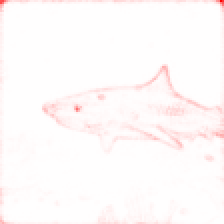
\includegraphics[width=\linewidth]{figures/experiments/saliency_quality/image_0018_ILSVRC2012_val_00034038.JPEG/zennit_lrp_gamma0.25_features_5_abs.png}
    \end{minipage}\hspace{0.002\linewidth}%
    \begin{minipage}[c]{0.10\linewidth}
        \centering
        
\includegraphics[width=\linewidth]{figures/experiments/saliency_quality/image_0018_ILSVRC2012_val_00034038.JPEG/hybrid_cam_shift_40_scale_max_winnerTakesItAllMaxpool_f14_cam_g.png}
    \end{minipage}\hspace{0.002\linewidth}%
    \begin{minipage}[c]{0.10\linewidth}
        \centering
        
\includegraphics[width=\linewidth]{figures/experiments/saliency_quality/image_0018_ILSVRC2012_val_00034038.JPEG/layer_cam_features_14_relu.png}
    \end{minipage}\hspace{0.002\linewidth}%
    \begin{minipage}[c]{0.10\linewidth}
        \centering
        
\includegraphics[width=\linewidth]{figures/experiments/saliency_quality/image_0018_ILSVRC2012_val_00034038.JPEG/hybrid_cam_shift_30_scale_max_winnerTakesItAllMaxpool_f26_cam_g_abs.png}
    \end{minipage}\hspace{0.002\linewidth}%
    \begin{minipage}[c]{0.10\linewidth}
        \centering
        
\includegraphics[width=\linewidth]{figures/experiments/saliency_quality/image_0018_ILSVRC2012_val_00034038.JPEG/layer_cam_features_26_relu.png}
    \end{minipage}\hspace{0.002\linewidth}%
    \begin{minipage}[c]{0.10\linewidth}
        \centering
        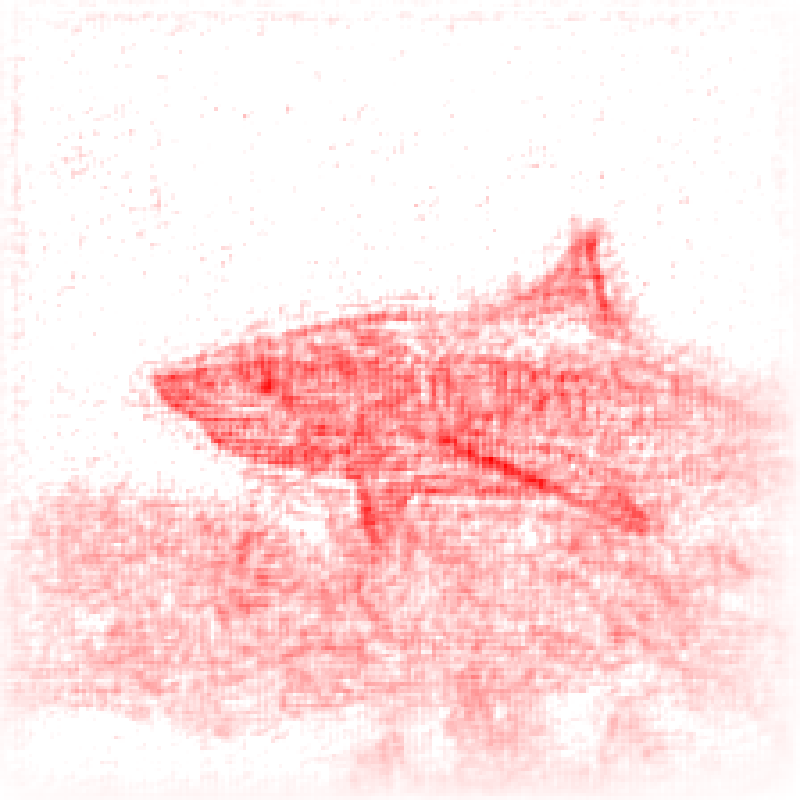
\includegraphics[width=\linewidth]{figures/experiments/saliency_quality/image_0018_ILSVRC2012_val_00034038.JPEG/hybrid_grad_shift_30_max_winnerTakesItAllMaxpool_f0_grad_pp.png}
    \end{minipage}%

    \vspace{0.3cm}

    \begin{minipage}[c]{0.08\linewidth}
        \centering
        \small goldfinch\\[1pt]
        {\scriptsize (1.0000)}
    \end{minipage}\hspace{0.002\linewidth}%
    \begin{minipage}[c]{0.10\linewidth}
        \centering
        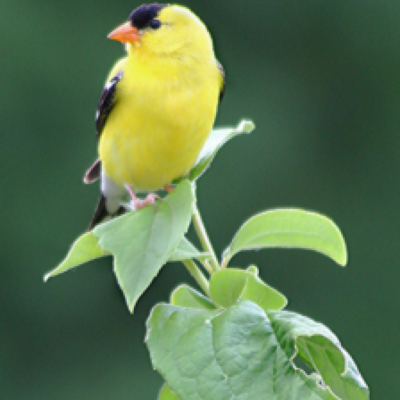
\includegraphics[width=\linewidth]{figures/experiments/saliency_quality/image_0034_ILSVRC2012_val_00044706.JPEG/original_image.png}
    \end{minipage}\hspace{0.002\linewidth}%
    \begin{minipage}[c]{0.10\linewidth}
        \centering
        
\includegraphics[width=\linewidth]{figures/experiments/saliency_quality/image_0034_ILSVRC2012_val_00044706.JPEG/hybrid_lrp_scaling_max_winnerTakesItAllMaxpool_f10_cam_pp_abs.png}
    \end{minipage}\hspace{0.002\linewidth}%
    \begin{minipage}[c]{0.10\linewidth}
        \centering
        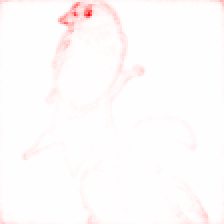
\includegraphics[width=\linewidth]{figures/experiments/saliency_quality/image_0034_ILSVRC2012_val_00044706.JPEG/zennit_lrp_gamma0.25_features_5_abs.png}
    \end{minipage}\hspace{0.002\linewidth}%
    \begin{minipage}[c]{0.10\linewidth}
        \centering
        
\includegraphics[width=\linewidth]{figures/experiments/saliency_quality/image_0034_ILSVRC2012_val_00044706.JPEG/hybrid_cam_shift_40_scale_max_winnerTakesItAllMaxpool_f14_cam_g.png}
    \end{minipage}\hspace{0.002\linewidth}%
    \begin{minipage}[c]{0.10\linewidth}
        \centering
        
\includegraphics[width=\linewidth]{figures/experiments/saliency_quality/image_0034_ILSVRC2012_val_00044706.JPEG/layer_cam_features_14_relu.png}
    \end{minipage}\hspace{0.002\linewidth}%
    \begin{minipage}[c]{0.10\linewidth}
        \centering
        
\includegraphics[width=\linewidth]{figures/experiments/saliency_quality/image_0034_ILSVRC2012_val_00044706.JPEG/hybrid_cam_shift_30_scale_max_winnerTakesItAllMaxpool_f26_cam_g_abs.png}
    \end{minipage}\hspace{0.002\linewidth}%
    \begin{minipage}[c]{0.10\linewidth}
        \centering
        
\includegraphics[width=\linewidth]{figures/experiments/saliency_quality/image_0034_ILSVRC2012_val_00044706.JPEG/layer_cam_features_26_relu.png}
    \end{minipage}\hspace{0.002\linewidth}%
    \begin{minipage}[c]{0.10\linewidth}
        \centering
        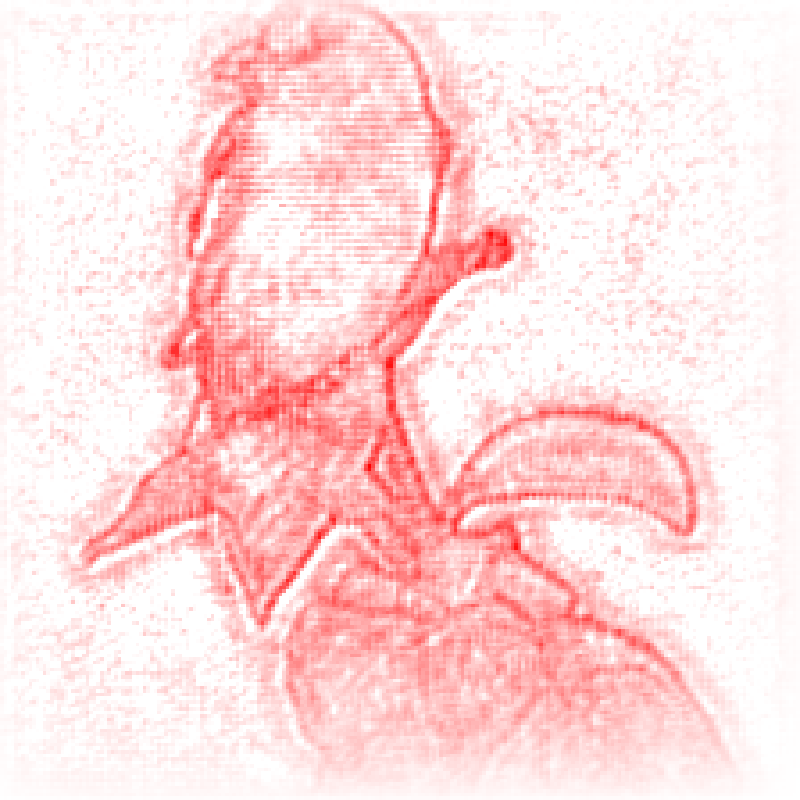
\includegraphics[width=\linewidth]{figures/experiments/saliency_quality/image_0034_ILSVRC2012_val_00044706.JPEG/hybrid_grad_shift_30_max_winnerTakesItAllMaxpool_f0_grad_pp.png}
    \end{minipage}%

    \vspace{0.3cm}

    \begin{minipage}[c]{0.08\linewidth}
        \centering
        \small tree frog\\[1pt]
        {\scriptsize (0.9954)}
    \end{minipage}\hspace{0.002\linewidth}%
    \begin{minipage}[c]{0.10\linewidth}
        \centering
        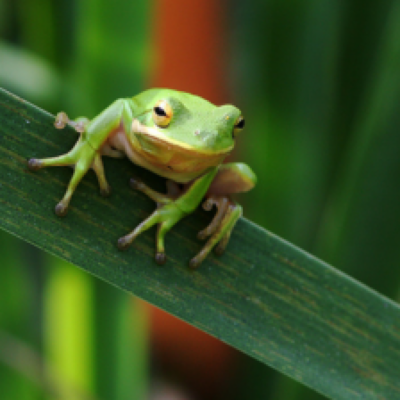
\includegraphics[width=\linewidth]{figures/experiments/saliency_quality/image_0041_ILSVRC2012_val_00017505.JPEG/original_image.png}
    \end{minipage}\hspace{0.002\linewidth}%
    \begin{minipage}[c]{0.10\linewidth}
        \centering
        
\includegraphics[width=\linewidth]{figures/experiments/saliency_quality/image_0041_ILSVRC2012_val_00017505.JPEG/hybrid_lrp_scaling_max_winnerTakesItAllMaxpool_f10_cam_pp_abs.png}
    \end{minipage}\hspace{0.002\linewidth}%
    \begin{minipage}[c]{0.10\linewidth}
        \centering
        
\includegraphics[width=\linewidth]{figures/experiments/saliency_quality/image_0041_ILSVRC2012_val_00017505.JPEG/zennit_lrp_gamma0.25_features_5_abs.png}
    \end{minipage}\hspace{0.002\linewidth}%
    \begin{minipage}[c]{0.10\linewidth}
        \centering
        
\includegraphics[width=\linewidth]{figures/experiments/saliency_quality/image_0041_ILSVRC2012_val_00017505.JPEG/hybrid_cam_shift_40_scale_max_winnerTakesItAllMaxpool_f14_cam_g.png}
    \end{minipage}\hspace{0.002\linewidth}%
    \begin{minipage}[c]{0.10\linewidth}
        \centering
        
\includegraphics[width=\linewidth]{figures/experiments/saliency_quality/image_0041_ILSVRC2012_val_00017505.JPEG/layer_cam_features_14_relu.png}
    \end{minipage}\hspace{0.002\linewidth}%
    \begin{minipage}[c]{0.10\linewidth}
        \centering
        
\includegraphics[width=\linewidth]{figures/experiments/saliency_quality/image_0041_ILSVRC2012_val_00017505.JPEG/hybrid_cam_shift_30_scale_max_winnerTakesItAllMaxpool_f26_cam_g_abs.png}
    \end{minipage}\hspace{0.002\linewidth}%
    \begin{minipage}[c]{0.10\linewidth}
        \centering
        
\includegraphics[width=\linewidth]{figures/experiments/saliency_quality/image_0041_ILSVRC2012_val_00017505.JPEG/layer_cam_features_26_relu.png}
    \end{minipage}\hspace{0.002\linewidth}%
    \begin{minipage}[c]{0.10\linewidth}
        \centering
        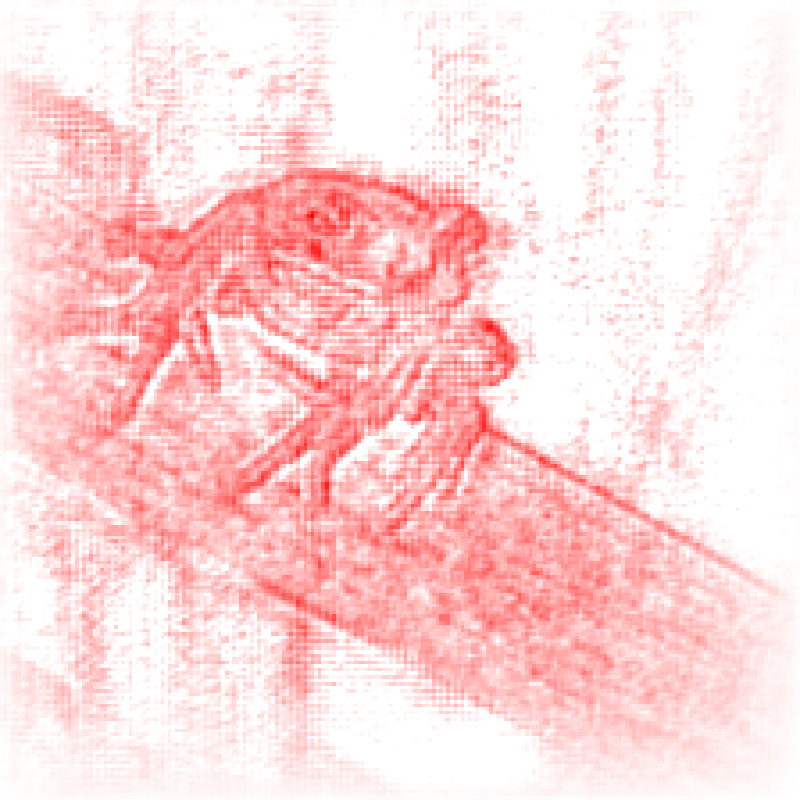
\includegraphics[width=\linewidth]{figures/experiments/saliency_quality/image_0041_ILSVRC2012_val_00017505.JPEG/hybrid_grad_shift_30_max_winnerTakesItAllMaxpool_f0_grad_pp.png}
    \end{minipage}%

    \vspace{0.3cm}

    \begin{minipage}[c]{0.08\linewidth}
        \centering
        \small ladybug\\[1pt]
        {\scriptsize (0.8272)}
    \end{minipage}\hspace{0.002\linewidth}%
    \begin{minipage}[c]{0.10\linewidth}
        \centering
        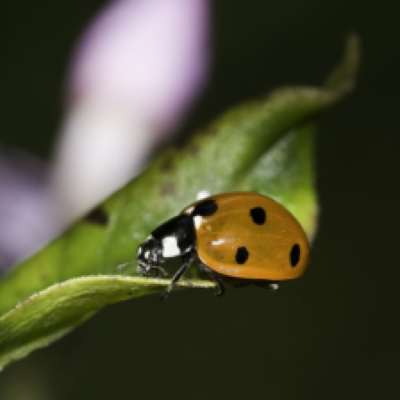
\includegraphics[width=\linewidth]{figures/experiments/saliency_quality/image_0096_ILSVRC2012_val_00025218.JPEG/original_image.png}
    \end{minipage}\hspace{0.002\linewidth}%
    \begin{minipage}[c]{0.10\linewidth}
        \centering
        
\includegraphics[width=\linewidth]{figures/experiments/saliency_quality/image_0096_ILSVRC2012_val_00025218.JPEG/hybrid_lrp_scaling_max_winnerTakesItAllMaxpool_f10_cam_pp_abs.png}
    \end{minipage}\hspace{0.002\linewidth}%
    \begin{minipage}[c]{0.10\linewidth}
        \centering
        
\includegraphics[width=\linewidth]{figures/experiments/saliency_quality/image_0096_ILSVRC2012_val_00025218.JPEG/zennit_lrp_gamma0.25_features_5_abs.png}
    \end{minipage}\hspace{0.002\linewidth}%
    \begin{minipage}[c]{0.10\linewidth}
        \centering
        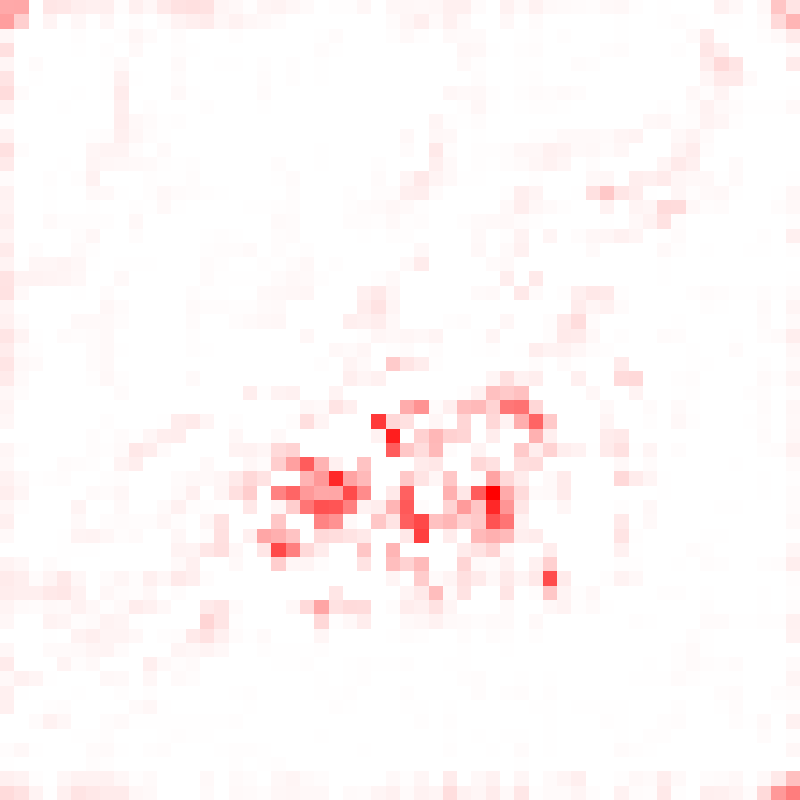
\includegraphics[width=\linewidth]{figures/experiments/saliency_quality/image_0096_ILSVRC2012_val_00025218.JPEG/hybrid_cam_shift_40_scale_max_winnerTakesItAllMaxpool_f14_cam_g.png}
    \end{minipage}\hspace{0.002\linewidth}%
    \begin{minipage}[c]{0.10\linewidth}
        \centering
        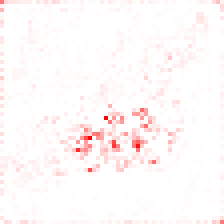
\includegraphics[width=\linewidth]{figures/experiments/saliency_quality/image_0096_ILSVRC2012_val_00025218.JPEG/layer_cam_features_14_relu.png}
    \end{minipage}\hspace{0.002\linewidth}%
    \begin{minipage}[c]{0.10\linewidth}
        \centering
        
\includegraphics[width=\linewidth]{figures/experiments/saliency_quality/image_0096_ILSVRC2012_val_00025218.JPEG/hybrid_cam_shift_30_scale_max_winnerTakesItAllMaxpool_f26_cam_g_abs.png}
    \end{minipage}\hspace{0.002\linewidth}%
    \begin{minipage}[c]{0.10\linewidth}
        \centering
        
\includegraphics[width=\linewidth]{figures/experiments/saliency_quality/image_0096_ILSVRC2012_val_00025218.JPEG/layer_cam_features_26_relu.png}
    \end{minipage}\hspace{0.002\linewidth}%
    \begin{minipage}[c]{0.10\linewidth}
        \centering
        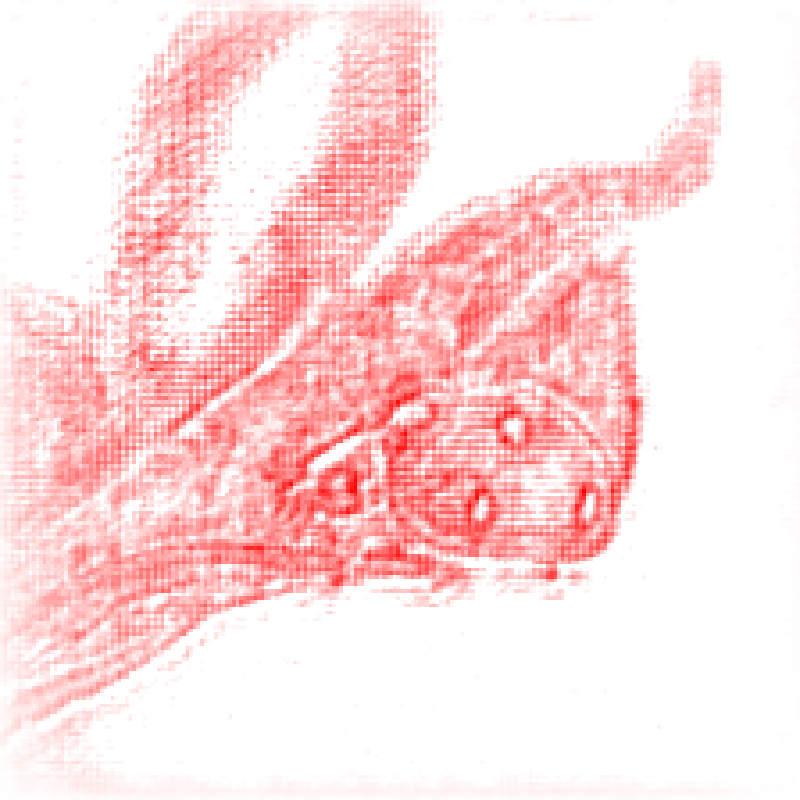
\includegraphics[width=\linewidth]{figures/experiments/saliency_quality/image_0096_ILSVRC2012_val_00025218.JPEG/hybrid_grad_shift_30_max_winnerTakesItAllMaxpool_f0_grad_pp.png}
    \end{minipage}%

    \vspace{0.3cm}

    \begin{minipage}[c]{0.08\linewidth}
        \centering
        \small wood rabbit\\[1pt]
        {\scriptsize (0.9782)}
    \end{minipage}\hspace{0.002\linewidth}%
    \begin{minipage}[c]{0.10\linewidth}
        \centering
        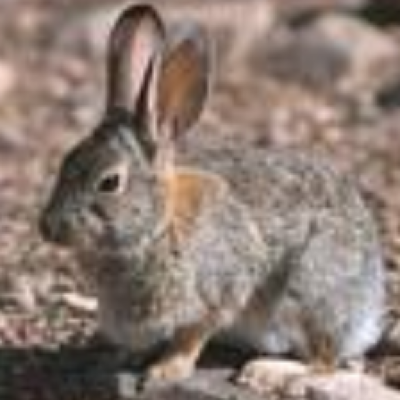
\includegraphics[width=\linewidth]{figures/experiments/saliency_quality/image_0120_ILSVRC2012_val_00024858.JPEG/original_image.png}
    \end{minipage}\hspace{0.002\linewidth}%
    \begin{minipage}[c]{0.10\linewidth}
        \centering
        
\includegraphics[width=\linewidth]{figures/experiments/saliency_quality/image_0120_ILSVRC2012_val_00024858.JPEG/hybrid_lrp_scaling_max_winnerTakesItAllMaxpool_f10_cam_pp_abs.png}
    \end{minipage}\hspace{0.002\linewidth}%
    \begin{minipage}[c]{0.10\linewidth}
        \centering
        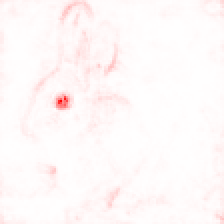
\includegraphics[width=\linewidth]{figures/experiments/saliency_quality/image_0120_ILSVRC2012_val_00024858.JPEG/zennit_lrp_gamma0.25_features_5_abs.png}
    \end{minipage}\hspace{0.002\linewidth}%
    \begin{minipage}[c]{0.10\linewidth}
        \centering
        
\includegraphics[width=\linewidth]{figures/experiments/saliency_quality/image_0120_ILSVRC2012_val_00024858.JPEG/hybrid_cam_shift_40_scale_max_winnerTakesItAllMaxpool_f14_cam_g.png}
    \end{minipage}\hspace{0.002\linewidth}%
    \begin{minipage}[c]{0.10\linewidth}
        \centering
        
\includegraphics[width=\linewidth]{figures/experiments/saliency_quality/image_0120_ILSVRC2012_val_00024858.JPEG/layer_cam_features_14_relu.png}
    \end{minipage}\hspace{0.002\linewidth}%
    \begin{minipage}[c]{0.10\linewidth}
        \centering
        
\includegraphics[width=\linewidth]{figures/experiments/saliency_quality/image_0120_ILSVRC2012_val_00024858.JPEG/hybrid_cam_shift_30_scale_max_winnerTakesItAllMaxpool_f26_cam_g_abs.png}
    \end{minipage}\hspace{0.002\linewidth}%
    \begin{minipage}[c]{0.10\linewidth}
        \centering
        
\includegraphics[width=\linewidth]{figures/experiments/saliency_quality/image_0120_ILSVRC2012_val_00024858.JPEG/layer_cam_features_26_relu.png}
    \end{minipage}\hspace{0.002\linewidth}%
    \begin{minipage}[c]{0.10\linewidth}
        \centering
        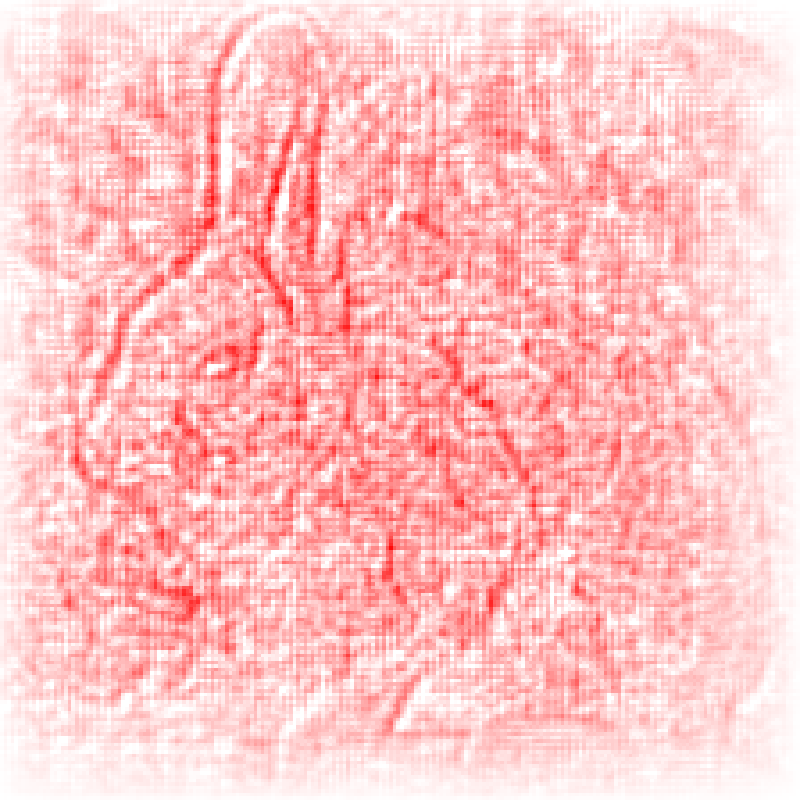
\includegraphics[width=\linewidth]{figures/experiments/saliency_quality/image_0120_ILSVRC2012_val_00024858.JPEG/hybrid_grad_shift_30_max_winnerTakesItAllMaxpool_f0_grad_pp.png}
    \end{minipage}%

    \vspace{0.3cm}

    \begin{minipage}[c]{0.08\linewidth}
        \centering
        \small water tower\\[1pt]
        {\scriptsize (1.0000)}
    \end{minipage}\hspace{0.002\linewidth}%
    \begin{minipage}[c]{0.10\linewidth}
        \centering
        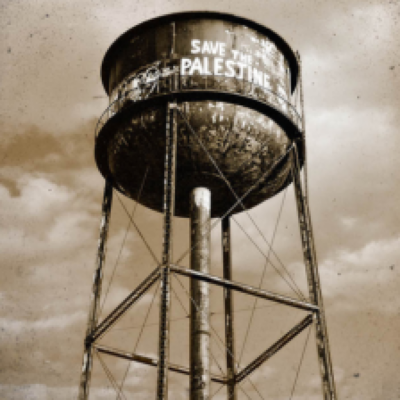
\includegraphics[width=\linewidth]{figures/experiments/saliency_quality/image_0499_ILSVRC2012_val_00037082.JPEG/original_image.png}
    \end{minipage}\hspace{0.002\linewidth}%
    \begin{minipage}[c]{0.10\linewidth}
        \centering
        
\includegraphics[width=\linewidth]{figures/experiments/saliency_quality/image_0499_ILSVRC2012_val_00037082.JPEG/hybrid_lrp_scaling_max_winnerTakesItAllMaxpool_f10_cam_pp_abs.png}
    \end{minipage}\hspace{0.002\linewidth}%
    \begin{minipage}[c]{0.10\linewidth}
        \centering
        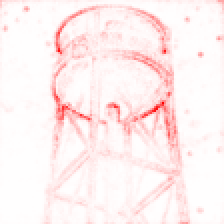
\includegraphics[width=\linewidth]{figures/experiments/saliency_quality/image_0499_ILSVRC2012_val_00037082.JPEG/zennit_lrp_gamma0.25_features_5_abs.png}
    \end{minipage}\hspace{0.002\linewidth}%
    \begin{minipage}[c]{0.10\linewidth}
        \centering
        
\includegraphics[width=\linewidth]{figures/experiments/saliency_quality/image_0499_ILSVRC2012_val_00037082.JPEG/hybrid_cam_shift_40_scale_max_winnerTakesItAllMaxpool_f14_cam_g.png}
    \end{minipage}\hspace{0.002\linewidth}%
    \begin{minipage}[c]{0.10\linewidth}
        \centering
        
\includegraphics[width=\linewidth]{figures/experiments/saliency_quality/image_0499_ILSVRC2012_val_00037082.JPEG/layer_cam_features_14_relu.png}
    \end{minipage}\hspace{0.002\linewidth}%
    \begin{minipage}[c]{0.10\linewidth}
        \centering
        
\includegraphics[width=\linewidth]{figures/experiments/saliency_quality/image_0499_ILSVRC2012_val_00037082.JPEG/hybrid_cam_shift_30_scale_max_winnerTakesItAllMaxpool_f26_cam_g_abs.png}
    \end{minipage}\hspace{0.002\linewidth}%
    \begin{minipage}[c]{0.10\linewidth}
        \centering
        
\includegraphics[width=\linewidth]{figures/experiments/saliency_quality/image_0499_ILSVRC2012_val_00037082.JPEG/layer_cam_features_26_relu.png}
    \end{minipage}\hspace{0.002\linewidth}%
    \begin{minipage}[c]{0.10\linewidth}
        \centering
        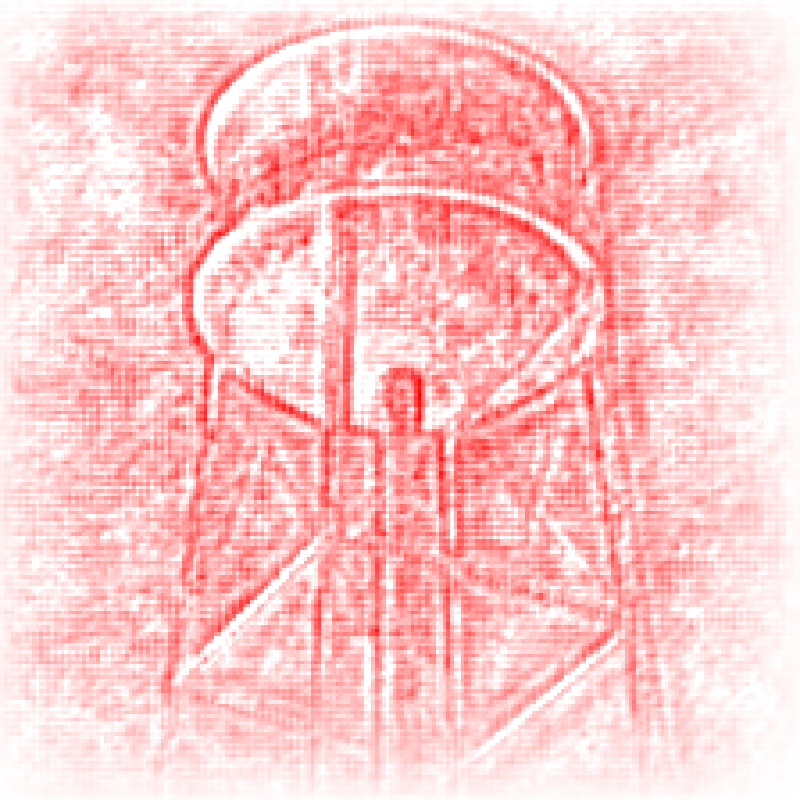
\includegraphics[width=\linewidth]{figures/experiments/saliency_quality/image_0499_ILSVRC2012_val_00037082.JPEG/hybrid_grad_shift_30_max_winnerTakesItAllMaxpool_f0_grad_pp.png}
    \end{minipage}%

    \vspace{0.3cm}

    \begin{minipage}[c]{0.08\linewidth}
        \centering
        \small yawl\\[1pt]
        {\scriptsize (0.9953)}
    \end{minipage}\hspace{0.002\linewidth}%
    \begin{minipage}[c]{0.10\linewidth}
        \centering
        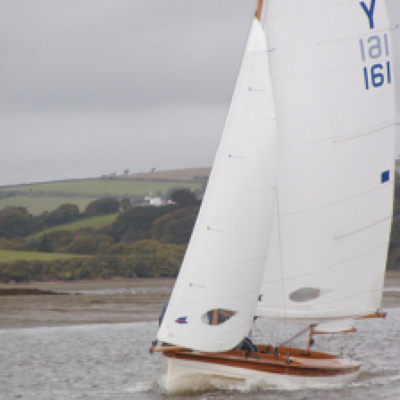
\includegraphics[width=\linewidth]{figures/experiments/saliency_quality/image_0511_ILSVRC2012_val_00035734.JPEG/original_image.png}
    \end{minipage}\hspace{0.002\linewidth}%
    \begin{minipage}[c]{0.10\linewidth}
        \centering
        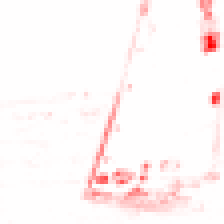
\includegraphics[width=\linewidth]{figures/experiments/saliency_quality/image_0511_ILSVRC2012_val_00035734.JPEG/hybrid_lrp_scaling_max_winnerTakesItAllMaxpool_f10_cam_pp_abs.png}
    \end{minipage}\hspace{0.002\linewidth}%
    \begin{minipage}[c]{0.10\linewidth}
        \centering
        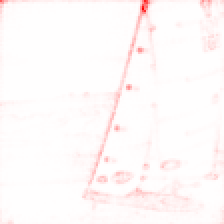
\includegraphics[width=\linewidth]{figures/experiments/saliency_quality/image_0511_ILSVRC2012_val_00035734.JPEG/zennit_lrp_gamma0.25_features_5_abs.png}
    \end{minipage}\hspace{0.002\linewidth}%
    \begin{minipage}[c]{0.10\linewidth}
        \centering
        
\includegraphics[width=\linewidth]{figures/experiments/saliency_quality/image_0511_ILSVRC2012_val_00035734.JPEG/hybrid_cam_shift_40_scale_max_winnerTakesItAllMaxpool_f14_cam_g.png}
    \end{minipage}\hspace{0.002\linewidth}%
    \begin{minipage}[c]{0.10\linewidth}
        \centering
        
\includegraphics[width=\linewidth]{figures/experiments/saliency_quality/image_0511_ILSVRC2012_val_00035734.JPEG/layer_cam_features_14_relu.png}
    \end{minipage}\hspace{0.002\linewidth}%
    \begin{minipage}[c]{0.10\linewidth}
        \centering
        
\includegraphics[width=\linewidth]{figures/experiments/saliency_quality/image_0511_ILSVRC2012_val_00035734.JPEG/hybrid_cam_shift_30_scale_max_winnerTakesItAllMaxpool_f26_cam_g_abs.png}
    \end{minipage}\hspace{0.002\linewidth}%
    \begin{minipage}[c]{0.10\linewidth}
        \centering
        
\includegraphics[width=\linewidth]{figures/experiments/saliency_quality/image_0511_ILSVRC2012_val_00035734.JPEG/layer_cam_features_26_relu.png}
    \end{minipage}\hspace{0.002\linewidth}%
    \begin{minipage}[c]{0.10\linewidth}
        \centering
        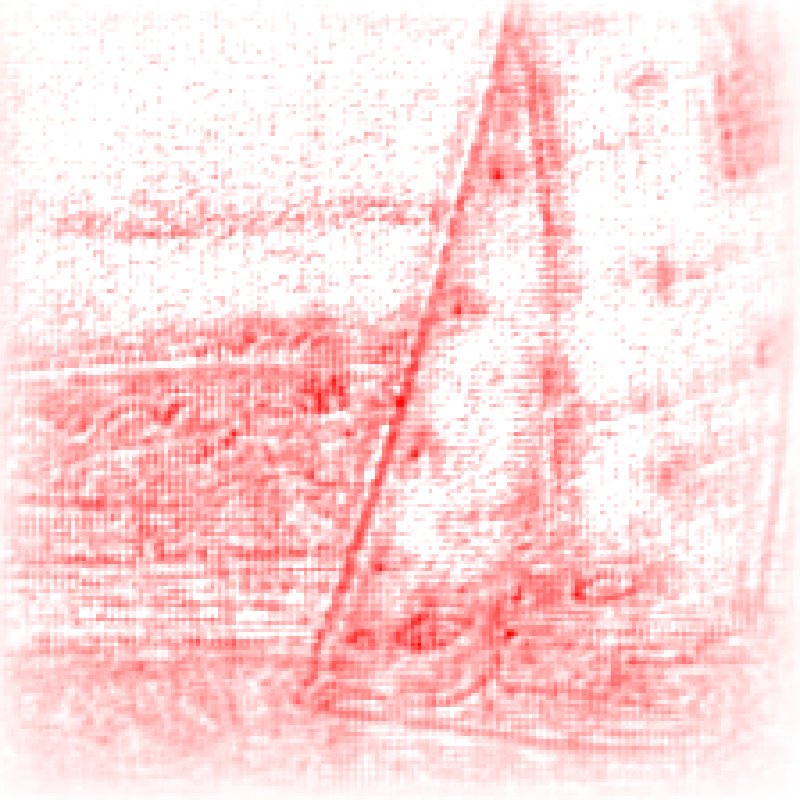
\includegraphics[width=\linewidth]{figures/experiments/saliency_quality/image_0511_ILSVRC2012_val_00035734.JPEG/hybrid_grad_shift_30_max_winnerTakesItAllMaxpool_f0_grad_pp.png}
    \end{minipage}%

    \caption{Saliency map comparison for VGG16 on images from the custom ImageNet-S test subset. Each row shows the predicted class (with confidence), original image, and saliency maps from different methods. Methods include SplitLRP, classical LRP, SplitCAM variants, LayerCAM, and SplitGrad.}
    \label{fig:vgg_saliency_comparison}
\end{figure}


\subsection{Quantitative Analysis on VGG-16}\label{app:vgg_split}

Table~\ref{tab:xai_eval_comprehensive_vgg} contains the complete VGG-16 comparison discussed in Section~\ref{sec:results_vgg}. Selected rows can differ in layer and absolute-value convention; the controlled $\alpha$ sweeps below isolate these choices more directly.

% Source: hiddenMonotonicity (Paper 1), appendix/table_appendix_generated_vgg_full_eval_sorted.tex — numbers verbatim.
\begingroup
\fontsize{8.5}{10}\selectfont
\setlength{\tabcolsep}{3pt}
\renewcommand{\arraystretch}{1.05}
\LongTableContent{
\caption[Comprehensive interpretability evaluation: VGG-16]{Comprehensive interpretability evaluation results (VGG-16; representative configurations, best per method). Abbreviations as in Table~\ref{tab:eval_vgg_main}. For each method configuration the best metric values across the considered layer configurations are highlighted in bold with dark blue shading. PF$^{\mathrm{drop}}$ is score-drop AUC; n/r denotes a result not reported in the paper, and n/a an inapplicable entry.}
    \label{tab:xai_eval_comprehensive_vgg}%
}{%
\begin{longtable}{@{}>{\raggedright\arraybackslash}p{3.6cm}cc cccccc@{}}
    \TableHeading \\
    \toprule
    Method & Layer & Abs & Sel$\downarrow$ & AL$\uparrow$ & PG$\uparrow$ & PF$^{\mathrm{drop}}_5$$\uparrow$ & PF$^{\mathrm{drop}}_{20}$$\uparrow$ & MaxS$\downarrow$ \\
    \midrule
    \endfirsthead

    \multicolumn{9}{c}%
    {{\tablename\ \thetable{} -- continued from previous page}} \\
    \toprule
    Method & Layer & Abs & Sel$\downarrow$ & AL$\uparrow$ & PG$\uparrow$ & PF$^{\mathrm{drop}}_5$$\uparrow$ & PF$^{\mathrm{drop}}_{20}$$\uparrow$ & MaxS$\downarrow$ \\
    \midrule
    \endhead

    \midrule
    \multicolumn{9}{r}{{Continued on next page}} \\
    \midrule
    \endfoot

    \bottomrule
    \endlastfoot

    \multicolumn{9}{c}{\textit{SplitCAM Methods}} \\
    \midrule
    SplitCAM (sc, $\alpha \ 0.4$) & (12, g) & n & 4.720 & \cellbest{\textbf{0.651}} & \cellbest{\textbf{0.912}} & 0.213 & 1.794 & \cellbest{\textbf{0.389}} \\
    SplitCAM (sc, $\alpha \ 0.4$) & (14, g) & n & \cellbest{\textbf{2.727}} & 0.563 & 0.836 & \cellbest{\textbf{0.300}} & \cellbest{\textbf{2.404}} & 1.012 \\
    \cmidrule(lr){1-9}
    SplitCAM (sc, $\alpha \ 0.4$, wta) & (14, g) & n & \cellbest{\textbf{2.761}} & 0.543 & 0.827 & \cellbest{\textbf{0.303}} & \cellbest{\textbf{2.414}} & 1.056 \\
    SplitCAM (sc, $\alpha \ 0.4$, wta) & (26, +, g) & y & 4.711 & \cellbest{\textbf{0.635}} & \cellbest{\textbf{0.938}} & 0.165 & 1.590 & \cellbest{\textbf{0.456}} \\
    \cmidrule(lr){1-9}
    SplitCAM (sc, $\alpha \ 0.5$, wta) & (14, g) & n & \cellbest{\textbf{2.766}} & 0.536 & 0.823 & \cellbest{\textbf{0.303}} & \cellbest{\textbf{2.416}} & 1.056 \\
    SplitCAM (sc, $\alpha \ 0.5$, wta) & (26, +, g) & n & 4.608 & \cellbest{\textbf{0.607}} & \cellbest{\textbf{0.903}} & 0.185 & 1.684 & \cellbest{\textbf{0.566}} \\
    \midrule
    \multicolumn{9}{c}{\textit{SplitGrad Methods}} \\
    \midrule
    SplitGrad ($\alpha \ 0.4$) & (12, +, g) & n & 5.633 & \cellbest{\textbf{0.613}} & \cellbest{\textbf{0.873}} & 0.148 & 1.461 & \cellbest{\textbf{0.364}} \\
    SplitGrad ($\alpha \ 0.4$) & (14, +, g) & y & \cellbest{\textbf{3.429}} & 0.533 & 0.820 & \cellbest{\textbf{0.235}} & \cellbest{\textbf{2.119}} & 0.851 \\
    \cmidrule(lr){1-9}
    SplitGrad ($\alpha \ 0.4$, wta) & (12, +, g) & n & 4.735 & \cellbest{\textbf{0.635}} & \cellbest{\textbf{0.883}} & 0.186 & 1.756 & 0.651 \\
    SplitGrad ($\alpha \ 0.4$, wta) & (14, +, g) & y & \cellbest{\textbf{3.287}} & 0.540 & 0.818 & \cellbest{\textbf{0.249}} & \cellbest{\textbf{2.186}} & 0.857 \\
    \cmidrule(lr){1-9}
    SplitGrad ($\alpha \ 0.5$, wta) & (12, +, g) & y & \cellbest{\textbf{3.379}} & \cellbest{\textbf{0.551}} & 0.859 & \cellbest{\textbf{0.261}} & \cellbest{\textbf{2.220}} & 0.869 \\
    SplitGrad ($\alpha \ 0.5$, wta) & (26, +, g) & y & 4.948 & 0.543 & \cellbest{\textbf{0.899}} & 0.162 & 1.527 & \cellbest{\textbf{0.617}} \\
    \midrule
    \multicolumn{9}{c}{\textit{SplitLRP Methods}} \\
    \midrule
    SplitLRP (sc) & (7, pos) & n & \cellbest{\textbf{3.062}} & 0.092 & \cellbest{\textbf{0.857}} & \cellbest{\textbf{0.296}} & \cellbest{\textbf{2.290}} & 0.865 \\
    SplitLRP (sc) & (19, pos) & n & 4.393 & \cellbest{\textbf{0.600}} & 0.823 & 0.166 & 1.656 & \cellbest{\textbf{0.291}} \\
    \cmidrule(lr){1-9}
    SplitLRP (sc, wta) & (7, pos) & n & \cellbest{\textbf{3.235}} & -0.036 & 0.836 & \cellbest{\textbf{0.296}} & \cellbest{\textbf{2.291}} & 0.866 \\
    SplitLRP (sc, wta) & (26, pos) & y & 5.168 & \cellbest{\textbf{0.588}} & \cellbest{\textbf{0.871}} & 0.151 & 1.473 & \cellbest{\textbf{0.282}} \\
    \midrule
    \multicolumn{9}{c}{\textit{Classical Methods (No Layer Optimization)}} \\
    \midrule
    Deconvolution & 0 & y & 5.435 & 0.468 & 0.629 & 0.204 & 1.715 & 0.956 \\
    DeepLIFT & 0 & y & 4.447 & 0.551 & 0.726 & 0.281 & 1.945 & 1.053 \\
    Feature Ablation & 0 & y & 6.029 & 0.479 & 0.624 & 0.123 & 1.250 & 0.859 \\
    GradientSHAP & 0 & y & 4.808 & 0.552 & 0.783 & 0.261 & 1.862 & 1.142 \\
    IntGrad & 0 & y & 4.838 & 0.554 & 0.797 & 0.262 & 1.851 & 1.069 \\
    Occlusion & 0 & y & 5.214 & 0.499 & 0.716 & 0.130 & 1.217 & 0.699 \\
    GCAM++ & 30 & n & 5.955 & 0.564 & 0.827 & 0.130 & 1.245 & 0.401 \\
    \midrule
    \multicolumn{9}{c}{\textit{Classical Methods (Layer Optimization)}} \\
    \midrule
    Guided Backprop & 2 & n & \cellbest{\textbf{3.276}} & \cellbest{\textbf{0.632}} & 0.883 & \cellbest{\textbf{0.281}} & \cellbest{\textbf{2.302}} & 0.571 \\
    Guided Backprop & 5 & n & 3.448 & 0.614 & \cellbest{\textbf{0.887}} & 0.240 & 2.091 & \cellbest{\textbf{0.375}} \\
    \cmidrule(lr){1-9}
    Guided GCAM & 0 & n & \cellbest{\textbf{4.301}} & \cellbest{\textbf{-0.053}} & \cellbest{\textbf{0.857}} & 0.161 & \cellbest{\textbf{1.459}} & 1.047 \\
    Guided GCAM & 26 & n & 5.130 & -2.635 & 0.843 & \cellbest{\textbf{0.179}} & 1.415 & \cellbest{\textbf{0.947}} \\
    \cmidrule(lr){1-9}
    GCAM & 0 & n & 6.006 & \cellbest{\textbf{0.356}} & \cellbest{\textbf{0.638}} & 0.060 & 0.899 & 1.123 \\
    GCAM & 14 & n & \cellbest{\textbf{5.555}} & 0.306 & 0.580 & \cellbest{\textbf{0.136}} & \cellbest{\textbf{1.525}} & \cellbest{\textbf{0.903}} \\
    \cmidrule(lr){1-9}
    LCAM & 14 & n/a & 2.792 & 0.576 & 0.798 & \cellbest{\textbf{0.317}} & \cellbest{\textbf{2.474}} & \cellbest{\textbf{2.656}} \\
    LCAM & 2 & n/a & \cellbest{\textbf{3.128}} & \cellbest{\textbf{0.580}} & \cellbest{\textbf{0.855}} & 0.300 & 2.191 & 5.508 \\
    \cmidrule(lr){1-9}
    LRP $\gamma=0.25$ & 0 & n & \cellbest{\textbf{3.189}} & \cellbest{\textbf{0.615}} & \cellbest{\textbf{0.680}} & 0.218 & 1.918 & 0.519 \\
    LRP $\gamma=0.25$ & 14 & n & 3.593 & 0.577 & 0.611 & \cellbest{\textbf{0.279}} & \cellbest{\textbf{2.255}} & \cellbest{\textbf{0.491}} \\
    \midrule
    \multicolumn{9}{c}{\textit{Baseline Methods}} \\
    \midrule
    Baseline: Binary Mask & 0 & y & 6.011 & 1.000 & 1.000 & 0.091 & 1.054 & n/r \\
    Baseline: Original Image & 0 & y & 8.770 & -1.699 & 0.572 & 0.061 & 0.619 & n/r \\
    Random Baseline & 0 & y & 3.570 & 0.425 & 0.458 & 0.203 & 1.585 & n/r \\
    \midrule
\end{longtable}%
}
\endgroup


\subsection{Quantitative Analysis on ResNet-18}\label{app:resnet_split}

Table~\ref{tab:xai_eval_comprehensive_res} reports all ResNet-18 split configurations, baselines and classical methods.

% Source: hiddenMonotonicity (Paper 1), appendix/table_appendix_generated_res_full_eval_sorted.tex — numbers verbatim.
% Note: the paper's appendix caption said "ResNet50"; the evaluated model is the ResNet18 of the
% main results (cf. tab:eval_res_main and the paper's main text), so the caption is corrected here.
\begin{longtable}{p{4cm}cc cccccc}
    \caption{Comprehensive interpretability evaluation results (ResNet-18; representative configurations, best per method). Abbreviations as in Table~\ref{tab:eval_res_main}. For each method configuration the best metric values across the considered layer configurations are highlighted in bold.}
    \label{tab:xai_eval_comprehensive_res} \\
    \toprule
    \textbf{Method} & \textbf{Layer} & \textbf{Abs} & \textbf{Select.} & \textbf{Attr. Loc.} & \textbf{Point.} & \textbf{Pixel Fl.} & \textbf{Pixel Fl.} & \textbf{Max Sens.} \\
     & & & \textbf{$\downarrow$} & \textbf{$\uparrow$} & \textbf{$\uparrow$} & \textbf{AUC@5 $\uparrow$} & \textbf{AUC@20 $\uparrow$} & \textbf{$\downarrow$} \\
    \midrule
    \endfirsthead

    \multicolumn{9}{c}%
    {{\tablename\ \thetable{} -- continued from previous page}} \\
    \toprule
    \textbf{Method} & \textbf{Layer} & \textbf{Abs} & \textbf{Select.} & \textbf{Attr. Loc.} & \textbf{Point.} & \textbf{Pixel Fl.} & \textbf{Pixel Fl.} & \textbf{Max Sens.} \\
     & & & \textbf{$\downarrow$} & \textbf{$\uparrow$} & \textbf{$\uparrow$} & \textbf{AUC@5 $\uparrow$} & \textbf{AUC@20 $\uparrow$} & \textbf{$\downarrow$} \\
    \midrule
    \endhead

    \midrule
    \multicolumn{9}{r}{{Continued on next page}} \\
    \midrule
    \endfoot

    \bottomrule
    \endlastfoot

    \multicolumn{9}{c}{\textit{SplitCAM Methods}} \\
    \midrule
    SplitCAM (sc, $\alpha\ 0.3$, wta) & (1.0.2, g) & n & \textbf{3.503} & 0.487 & 0.747 & \textbf{0.168} & \textbf{1.395} & 1.277 \\
    SplitCAM (sc, $\alpha\ 0.3$, wta) & (4.1.2, g) & n & 5.654 & \textbf{0.673} & \textbf{0.972} & 0.081 & 0.880 & \textbf{0.233} \\
    \cmidrule(lr){1-9}
    SplitCAM (sc, $\alpha\ 0.5$, wta) & (2.0.1, g) & n & \textbf{3.682} & -1.370 & 0.887 & \textbf{0.158} & \textbf{1.447} & 1.078 \\
    SplitCAM (sc, $\alpha\ 0.5$, wta) & (4.1.1, +, g) & y & 6.526 & \textbf{0.611} & \textbf{0.956} & 0.066 & 0.737 & \textbf{0.187} \\
    \midrule
    \multicolumn{9}{c}{\textit{SplitGrad Methods}} \\
    \midrule
    SplitGrad ($\alpha\ 0.3$, wta) & (1.0.2, g) & y & \textbf{4.449} & 0.513 & 0.777 & \textbf{0.149} & \textbf{1.266} & 0.813 \\
    SplitGrad ($\alpha\ 0.3$, wta) & (4.1.2, g) & y & 5.663 & \textbf{0.649} & \textbf{0.972} & 0.082 & 0.882 & \textbf{0.219} \\
    \cmidrule(lr){1-9}
    SplitGrad ($\alpha\ 0.5$, wta) & (3.1.1, g) & y & \textbf{3.588} & 0.559 & 0.880 & \textbf{0.130} & \textbf{1.366} & 0.859 \\
    SplitGrad ($\alpha\ 0.5$, wta) & (4.1.2, g) & y & 5.690 & \textbf{0.654} & \textbf{0.972} & 0.083 & 0.886 & \textbf{0.230} \\
    \midrule
    \multicolumn{9}{c}{\textit{SplitLRP Methods}} \\
    \midrule
    SplitLRP (sc, wta) & (conv1, pos) & y & \textbf{6.313} & \textbf{0.506} & \textbf{0.587} & \textbf{0.056} & \textbf{0.697} & 0.755 \\
    SplitLRP (sc, wta) & (1.0.2, pos) & y & 6.785 & 0.483 & 0.567 & 0.050 & 0.686 & \textbf{0.696} \\
    \midrule
    \multicolumn{9}{c}{\textit{Classical Methods (No Layer Optimization)}} \\
    \midrule
    Deconvolution & conv1 & y & 5.474 & 0.478 & 0.666 & 0.151 & 1.177 & 0.618 \\
    Gradient SHAP & conv1 & y & 5.269 & 0.527 & 0.779 & 0.166 & 1.227 & 1.074 \\
    GradCAM++ & 4.1.2 & n & 6.054 & 0.556 & 0.945 & 0.077 & 0.838 & 0.140 \\
    Integrated Gradients & conv1 & y & 5.265 & 0.528 & 0.777 & 0.167 & 1.226 & 0.994 \\
    Feature Ablation & conv1 & n & 4.655 & 0.136 & 0.684 & 0.188 & 1.388 & 1.077 \\
    Occlusion & conv1 & n & 5.300 & 0.179 & 0.726 & 0.130 & 1.030 & 0.785 \\
    Deconvolution & conv1 & n & 3.934 & 0.484 & 0.666 & 0.147 & 1.203 & 0.751 \\
    \midrule
    \multicolumn{9}{c}{\textit{Classical Methods (Layer Optimization)}} \\
    \midrule
    GradCAM & 2.0.1 & y & \textbf{4.003} & 0.450 & 0.678 & 0.052 & \textbf{1.024} & 0.738 \\
    GradCAM & 4.1.2 & n & 6.070 & \textbf{0.554} & \textbf{0.945} & \textbf{0.076} & 0.829 & \textbf{0.131} \\
    \cmidrule(lr){1-9}
    Guided GradCAM & 4.0.2 & n & 4.929 & \textbf{0.742} & 0.866 & 0.119 & 1.008 & 0.687 \\
    Guided GradCAM & 4.1.2 & n & \textbf{3.843} & 0.717 & \textbf{0.883} & \textbf{0.129} & \textbf{1.096} & \textbf{0.612} \\
    \cmidrule(lr){1-9}
    LayerCAM & 2.0.2 & n & \textbf{3.690} & 0.549 & 0.865 & \textbf{0.144} & \textbf{1.428} & 0.913 \\
    LayerCAM & 4.1.1 & n & 5.661 & \textbf{0.664} & \textbf{0.971} & 0.083 & 0.890 & \textbf{0.227} \\
    \cmidrule(lr){1-9}
    LRP $\gamma=0.25$ & conv1 & y & \textbf{3.550} & \textbf{0.656} & 0.852 & \textbf{0.213} & \textbf{1.737} & 0.521 \\
    LRP $\gamma=0.25$ & 4.1.1 & n & 5.649 & 0.630 & \textbf{0.965} & 0.081 & 0.877 & \textbf{0.200} \\
    \cmidrule(lr){1-9}
    Guided Backprop & conv1 & n & \textbf{3.517} & \textbf{0.621} & 0.867 & \textbf{0.212} & \textbf{1.757} & 0.459 \\
    Guided Backprop & 3.1.2 & n & 3.874 & 0.582 & \textbf{0.938} & 0.121 & 1.307 & \textbf{0.213} \\
    \midrule
    \multicolumn{9}{c}{\textit{Baseline Methods}} \\
    \midrule
    Baseline: Original Image & conv1 & y & 8.351 & -1.699 & 0.572 & 0.049 & 0.435 & -- \\
    Baseline: Binary Mask & conv1 & y & 5.964 & 1.000 & 1.000 & 0.067 & 0.739 & -- \\
    Random Baseline & - & y & 4.071 & 0.425 & 0.440 & 0.147 & 1.067 & -- \\
    \midrule
    \end{longtable}


\section{Stabilization Ablations for the Split Methods}\label{app:ablation}

These ablations examine forward/backward stabilization and the max-pooling implementation (Section~\ref{sec:stabilization_dc}).

\subsection{Backward-Pass Stabilization}\label{app:backward_ablation}

Table~\ref{tab:alpha_comparison_by_method} gives the full $\alpha$ grid underlying Section~\ref{subsec:alpha_ablation}. Layer-14 configurations show smaller or adverse changes in some metrics. Convex and winner-takes-it-all max-pooling differ little near $\alpha=0.5$ and more at lower values; their ranking depends on configuration and metric.

\paragraph{Unresolved source-table discrepancy.}
For SplitCAM with scaling, $\alpha=0.4$, winner-takes-it-all pooling and absolute-value configuration $(26,+,g)$, Table~\ref{tab:xai_eval_comprehensive_vgg} reports PF$^{\mathrm{drop}}_{20}=1.590$ and MaxS$=0.456$, versus $1.5849$ and $0.4573$ in Table~\ref{tab:alpha_comparison_by_method}. These source-table values remain unchanged: the per-image results needed to resolve their discrepancy are unavailable, leaving its cause unknown.

% Source: hiddenMonotonicity (Paper 1), appendix/table_ppendix_alpha_combined.tex — numbers verbatim, restyled to booktabs.
\begin{table}[htb!]
    \centering
    \footnotesize
    \setlength{\tabcolsep}{5pt}
    \renewcommand{\arraystretch}{1.2}
    \caption[Alpha ablation for SplitGrad and SplitCAM]{Alpha ablation as performed in Section~\ref{sec:ablations} across four SplitGrad and SplitCAM configurations of layers $14$ and $26$, respectively. The notation is similar to Table~\ref{tab:eval_vgg_main}.}
    \label{tab:alpha_comparison_by_method}\label{tab:alpha_ablation_main}
\TableContent{
    \begin{adjustbox}{max width=\linewidth}
\begin{tabular}{ll cccccc}
    \toprule
    \textbf{Method} & \textbf{Metric} & $\alpha \ 0.50$ & $\alpha \ 0.45$ & $\alpha \ 0.40$ & $\alpha \ 0.35$ & $\alpha \ 0.30$ & $\alpha \ 0.00$ \\
    \midrule
    \multirow{4}{*}{\begin{tabular}[c]{@{}l@{}}\textbf{SplitGrad (wta)}\\(26, g), abs\end{tabular}} & PG$\uparrow$ & 0.8975 & 0.9064 & 0.9470 & \cellbest{\textbf{0.9558}} & 0.8887 & 0.4011 \\
     & AL$\uparrow$ & 0.5434 & 0.5476 & 0.6051 & \cellbest{\textbf{0.6169}} & 0.5346 & 0.4486 \\
     & MaxS$\downarrow$ & 0.6160 & 0.6071 & 0.4399 & 0.2382 & 0.3344 & \cellbest{\textbf{0.0283}} \\
     & PF$^{\mathrm{drop}}_{20}$ $\uparrow$ & 1.5270 & 1.5337 & \cellbest{\textbf{1.5808}} & 1.4476 & 1.3171 & 1.2471 \\
    \midrule
    \multirow{4}{*}{\begin{tabular}[c]{@{}l@{}}\textbf{SplitGrad}\\(26, g), abs\end{tabular}} & PG$\uparrow$ & 0.8975 & 0.9064 & \cellbest{\textbf{0.9470}} & 0.9099 & 0.2827 & 0.6413 \\
     & AL$\uparrow$ & 0.5434 & 0.5476 & \cellbest{\textbf{0.6037}} & 0.5216 & 0.4245 & 0.4563 \\
     & MaxS$\downarrow$ & 0.6171 & 0.6102 & 0.4426 & 0.3864 & 0.0622 & \cellbest{\textbf{0.0079}} \\
     & PF$^{\mathrm{drop}}_{20}$ $\uparrow$ & 1.5272 & 1.5333 & \cellbest{\textbf{1.5876}} & 1.3702 & 0.2431 & 0.5755 \\
    \midrule
    \multirow{4}{*}{\begin{tabular}[c]{@{}l@{}}\textbf{SplitGrad (wta)}\\(14, g), abs\end{tabular}} & PG$\uparrow$ & 0.8198 & 0.8198 & 0.8198 & \cellbest{\textbf{0.8322}} & 0.8127 & 0.7898 \\
     & AL$\uparrow$ & \cellbest{\textbf{0.5403}} & 0.5403 & 0.5402 & 0.5006 & 0.4936 & 0.4857 \\
     & MaxS$\downarrow$ & 0.8579 & 0.8597 & 0.8584 & 0.0875 & 0.0677 & \cellbest{\textbf{0.0481}} \\
     & PF$^{\mathrm{drop}}_{20}$ $\uparrow$ & 2.1887 & \cellbest{\textbf{2.1894}} & 2.1869 & 1.8740 & 1.8304 & 1.7684 \\
    \midrule
    \multirow{4}{*}{\begin{tabular}[c]{@{}l@{}}\textbf{SplitGrad}\\(14, g), abs\end{tabular}} & PG$\uparrow$ & 0.8198 & \cellbest{\textbf{0.8198}} & 0.8180 & 0.7951 & 0.8004 & 0.7968 \\
     & AL$\uparrow$ & 0.5403 & \cellbest{\textbf{0.5403}} & 0.5330 & 0.5054 & 0.4926 & 0.4847 \\
     & MaxS$\downarrow$ & 0.8618 & 0.8584 & 0.8478 & 0.1103 & 0.0662 & \cellbest{\textbf{0.0301}} \\
     & PF$^{\mathrm{drop}}_{20}$ $\uparrow$ & \cellbest{\textbf{2.1894}} & 2.1891 & 2.1185 & 1.3425 & 1.2959 & 1.1927 \\
    \midrule
    \multirow{4}{*}{\begin{tabular}[c]{@{}l@{}}\textbf{SplitCAM (sc, wta)}\\(26, +, g), abs\end{tabular}} & PG$\uparrow$ & 0.8675 & 0.8675 & \cellbest{\textbf{0.9382}} & 0.9329 & 0.6131 & 0.8551 \\
     & AL$\uparrow$ & 0.5501 & 0.5535 & 0.6347 & \cellbest{\textbf{0.6627}} & 0.4033 & 0.5133 \\
     & MaxS$\downarrow$ & 0.6906 & 0.6820 & 0.4573 & 0.2645 & 0.2511 & \cellbest{\textbf{0.1196}} \\
     & PF$^{\mathrm{drop}}_{20}$ $\uparrow$ & 1.6067 & \cellbest{\textbf{1.6085}} & 1.5849 & 1.4989 & 0.8534 & 1.5071 \\
    \midrule
    \multirow{4}{*}{\begin{tabular}[c]{@{}l@{}}\textbf{SplitCAM (sc)}\\(26, +, g), abs\end{tabular}} & PG$\uparrow$ & 0.8940 & 0.8905 & \cellbest{\textbf{0.9346}} & 0.6466 & 0.8251 & 0.8604 \\
     & AL$\uparrow$ & 0.5595 & 0.5636 & \cellbest{\textbf{0.6363}} & 0.4015 & 0.4977 & 0.5114 \\
     & MaxS$\downarrow$ & 0.6738 & 0.6640 & 0.4520 & 0.3729 & 0.1102 & \cellbest{\textbf{0.1062}} \\
     & PF$^{\mathrm{drop}}_{20}$ $\uparrow$ & 1.5902 & \cellbest{\textbf{1.5978}} & 1.5906 & 0.9076 & 1.2784 & 1.3605 \\
    \midrule
    \multirow{4}{*}{\begin{tabular}[c]{@{}l@{}}\textbf{SplitCAM (sc, wta)}\\(14, g)\end{tabular}} & PG$\uparrow$ & 0.8251 & 0.8251 & \cellbest{\textbf{0.8269}} & 0.7880 & 0.7809 & 0.7703 \\
     & AL$\uparrow$ & 0.5363 & 0.5363 & \cellbest{\textbf{0.5435}} & 0.5338 & 0.5286 & 0.5225 \\
     & MaxS$\downarrow$ & 1.0566 & 1.0569 & 1.0489 & \cellbest{\textbf{0.1620}} & 0.1625 & 0.1630 \\
     & PF$^{\mathrm{drop}}_{20}$ $\uparrow$ & 2.4128 & 2.4130 & \cellbest{\textbf{2.4135}} & 1.9014 & 1.8613 & 1.8731 \\
    \midrule
    \multirow{4}{*}{\begin{tabular}[c]{@{}l@{}}\textbf{SplitCAM (sc)}\\(14, g)\end{tabular}} & PG$\uparrow$ & 0.8251 & 0.8251 & \cellbest{\textbf{0.8428}} & 0.7756 & 0.7686 & 0.7756 \\
     & AL$\uparrow$ & 0.5363 & 0.5363 & \cellbest{\textbf{0.5626}} & 0.5363 & 0.5271 & 0.5208 \\
     & MaxS$\downarrow$ & 1.0552 & 1.0593 & 1.0136 & 0.1629 & 0.1585 & \cellbest{\textbf{0.1555}} \\
     & PF$^{\mathrm{drop}}_{20}$ $\uparrow$ & 2.4171 & \cellbest{\textbf{2.4172}} & 2.4065 & 1.5032 & 1.5082 & 1.5139 \\
    \bottomrule
    \end{tabular}
\end{adjustbox}
}%
\end{table}


\subsection{Forward-stabilization grids}

Tables~\ref{tab:alpha_comparison_none} and~\ref{tab:alpha_comparison_shift} give the full unstabilized and shift-stabilized SplitCAM grids discussed in Section~\ref{app:forward_ablation}.

% Source: hiddenMonotonicity (Paper 1), appendix/table_alpha_none.tex — numbers verbatim, restyled to booktabs.
% The paper's green cell highlighting is rendered here as a star marker (*) since the thesis
% preamble does not load colortbl.
\begin{table}[htbp]
    \centering
    \footnotesize
    \setlength{\tabcolsep}{5pt}
    \renewcommand{\arraystretch}{1.2}
    \caption[Alpha ablation without forward stabilization]{Alpha ablation for scale normalization across four SplitCAM configurations of layers 14 and 26. Here, in the forward pass \emph{no} stabilization is applied. Notation and structure are similar to Table~\ref{tab:alpha_comparison_by_method}. Light blue entries marked with $^{\ast}$ indicate better performance of the method compared to the default variant with scale stabilization in the forward pass.}
    \label{tab:alpha_comparison_none}
    \begin{adjustbox}{max width=\linewidth}
\begin{tabular}{ll cccccc}
    \toprule
    \textbf{Method} & \textbf{Metric} & $\alpha \ 0.50$ & $\alpha \ 0.45$ & $\alpha \ 0.40$ & $\alpha \ 0.35$ & $\alpha \ 0.30$ & $\alpha \ 0.00$ \\
    \midrule
    \multirow{4}{*}{\begin{tabular}[c]{@{}l@{}}\textbf{SplitCAM (sc, wta)}\\(26, +, g), abs\end{tabular}} & PG$\uparrow$ & 0.7686 & 0.7686 & 0.8632 & \cellbest{\textbf{0.8712}} & 0.3441 & 0.5453 \\
     & AL$\uparrow$ & 0.5374 & 0.5412 & 0.5943 & \cellbest{\textbf{0.6118}} & 0.3595 & 0.4569 \\
     & MaxS$\downarrow$ & \cellapprox{0.6578}$^{\ast}$ & \cellapprox{0.6507}$^{\ast}$ & 0.4841 & 0.2873 & \cellapprox{0.1918}$^{\ast}$ & \cellapprox{\cellbest{\textbf{0.0135}}}$^{\ast}$ \\
     & PF$^{\mathrm{drop}}_{20}$ $\uparrow$ & 1.2744 & 1.2859 & \cellbest{\textbf{1.3209}} & 1.1792 & 0.4430 & 0.6527 \\
    \midrule
    \multirow{4}{*}{\begin{tabular}[c]{@{}l@{}}\textbf{SplitCAM (sc)}\\(26, +, g), abs\end{tabular}} & PG$\uparrow$ & 0.7565 & 0.7565 & \cellbest{\textbf{0.8451}} & 0.3783 & 0.4507 & 0.4970 \\
     & AL$\uparrow$ & 0.5346 & 0.5384 & \cellbest{\textbf{0.5897}} & 0.3663 & 0.4420 & 0.4545 \\
     & MaxS$\downarrow$ & \cellapprox{0.6604}$^{\ast}$ & \cellapprox{0.6512}$^{\ast}$ & 0.4985 & \cellapprox{0.3077}$^{\ast}$ & \cellapprox{0.0279}$^{\ast}$ & \cellapprox{\cellbest{\textbf{0.0043}}}$^{\ast}$ \\
     & PF$^{\mathrm{drop}}_{20}$ $\uparrow$ & 1.2680 & 1.2856 & \cellbest{\textbf{1.3295}} & 0.5912 & 0.4906 & 0.5563 \\
    \midrule
    \multirow{4}{*}{\begin{tabular}[c]{@{}l@{}}\textbf{SplitCAM (sc, wta)}\\(14, g)\end{tabular}} & PG$\uparrow$ & \cellapprox{\cellbest{\textbf{0.8491}}}$^{\ast}$ & \cellapprox{0.8491}$^{\ast}$ & \cellapprox{0.8491}$^{\ast}$ & 0.7867 & \cellapprox{0.7847}$^{\ast}$ & 0.7686 \\
     & AL$\uparrow$ & 0.5324 & 0.5321 & \cellbest{\textbf{0.5406}} & 0.5306 & 0.5261 & 0.5200 \\
     & MaxS$\downarrow$ & 1.0834 & 1.0814 & 1.0885 & \cellbest{\textbf{0.2271}} & 0.2309 & 0.2384 \\
     & PF$^{\mathrm{drop}}_{20}$ $\uparrow$ & \cellapprox{2.4454}$^{\ast}$ & \cellapprox{2.4482}$^{\ast}$ & \cellapprox{\cellbest{\textbf{2.4486}}}$^{\ast}$ & \cellapprox{1.9588}$^{\ast}$ & \cellapprox{1.9193}$^{\ast}$ & \cellapprox{1.9349}$^{\ast}$ \\
    \midrule
    \multirow{4}{*}{\begin{tabular}[c]{@{}l@{}}\textbf{SplitCAM (sc)}\\(14, g)\end{tabular}} & PG$\uparrow$ & 0.7746 & 0.7767 & \cellbest{\textbf{0.7847}} & 0.5855 & 0.5594 & 0.5573 \\
     & AL$\uparrow$ & 0.4003 & 0.4144 & \cellbest{\textbf{0.5517}} & 0.5300 & 0.5209 & 0.5137 \\
     & MaxS$\downarrow$ & 1.5733 & 1.5627 & 1.5443 & \cellbest{\textbf{1.2661}} & 1.3939 & 1.4272 \\
     & PF$^{\mathrm{drop}}_{20}$ $\uparrow$ & 2.1298 & \cellbest{\textbf{2.1384}} & 2.1371 & \cellapprox{1.6669}$^{\ast}$ & \cellapprox{1.6793}$^{\ast}$ & \cellapprox{1.6740}$^{\ast}$ \\
    \bottomrule
    \end{tabular}
\end{adjustbox}
\end{table}

% Source: hiddenMonotonicity (Paper 1), appendix/table_alpha_shift.tex — numbers verbatim, restyled to booktabs.
% The paper's green cell highlighting is rendered here as a star marker (*) since the thesis
% preamble does not load colortbl.
\begin{table}[htbp]
    \centering
    \footnotesize
    \setlength{\tabcolsep}{5pt}
    \renewcommand{\arraystretch}{1.2}
    \caption{Alpha ablation for scaling normalization across four SplitCAM configurations of layers 14 and 26. Here, in the forward pass shift normalization is applied. Notation and structure are similar to Table~\ref{tab:alpha_comparison_by_method}. Entries marked with $^{\ast}$ indicate better performance of the method compared to the default variant with scale stabilization in the forward pass.}
    \label{tab:alpha_comparison_shift}
    \begin{tabular}{ll cccccc}
    \toprule
    \textbf{Method} & \textbf{Metric} & $\alpha \ 0.50$ & $\alpha \ 0.45$ & $\alpha \ 0.40$ & $\alpha \ 0.35$ & $\alpha \ 0.30$ & $\alpha \ 0.00$ \\
    \midrule
    \multirow{4}{*}{\begin{tabular}[c]{@{}l@{}}\textbf{SplitCAM (sc, wta)}\\(26, +, g), abs\end{tabular}} & Point. $\uparrow$ & 0.8330 & 0.8149 & 0.7968 & \textbf{0.9235} & 0.6036 & 0.8592$^{\ast}$ \\
     & Attr. Loc. $\uparrow$ & 0.5242 & 0.5203 & 0.5147 & \textbf{0.6549} & 0.3968 & 0.5093 \\
     & Max Sens. $\downarrow$ & 0.6180$^{\ast}$ & 0.6182$^{\ast}$ & 0.6509 & 0.3104 & 0.2791 & \textbf{0.1665} \\
     & Pixel Fl. @20 $\uparrow$ & \textbf{1.6804}$^{\ast}$ & 1.6646$^{\ast}$ & 1.5065 & 1.4962 & 0.8896$^{\ast}$ & 1.5405$^{\ast}$ \\
    \midrule
    \multirow{4}{*}{\begin{tabular}[c]{@{}l@{}}\textbf{SplitCAM (sc)}\\(26, +, g), abs\end{tabular}} & Point. $\uparrow$ & 0.8330 & 0.8149 & 0.7988 & 0.5654 & 0.8431$^{\ast}$ & \textbf{0.8652}$^{\ast}$ \\
     & Attr. Loc. $\uparrow$ & \textbf{0.5242} & 0.5203 & 0.5076 & 0.3736 & 0.4949 & 0.5094 \\
     & Max Sens. $\downarrow$ & 0.6129$^{\ast}$ & 0.6168$^{\ast}$ & 0.6494 & 0.3820 & 0.1686 & \textbf{0.1664} \\
     & Pixel Fl. @20 $\uparrow$ & \textbf{1.6804}$^{\ast}$ & 1.6646$^{\ast}$ & 1.5105 & 0.8714 & 1.4289$^{\ast}$ & 1.4765$^{\ast}$ \\
    \midrule
    \multirow{4}{*}{\begin{tabular}[c]{@{}l@{}}\textbf{SplitCAM (sc, wta)}\\(14, g)\end{tabular}} & Point. $\uparrow$ & \textbf{0.8310}$^{\ast}$ & 0.8310$^{\ast}$ & 0.8310$^{\ast}$ & 0.7887$^{\ast}$ & 0.7827$^{\ast}$ & 0.7726$^{\ast}$ \\
     & Attr. Loc. $\uparrow$ & 0.5312 & 0.5312 & \textbf{0.5376} & 0.5315 & 0.5264 & 0.5203 \\
     & Max Sens. $\downarrow$ & 1.0562$^{\ast}$ & 1.0521$^{\ast}$ & 1.0649 & \textbf{0.1633} & 0.1641 & 0.1642 \\
     & Pixel Fl. @20 $\uparrow$ & \textbf{2.4412}$^{\ast}$ & 2.4412$^{\ast}$ & 2.4400$^{\ast}$ & 1.9306$^{\ast}$ & 1.8953$^{\ast}$ & 1.9059$^{\ast}$ \\
    \midrule
    \multirow{4}{*}{\begin{tabular}[c]{@{}l@{}}\textbf{SplitCAM (sc)}\\(14, g)\end{tabular}} & Point. $\uparrow$ & 0.8310$^{\ast}$ & 0.8310$^{\ast}$ & \textbf{0.8431}$^{\ast}$ & 0.7746 & 0.7706$^{\ast}$ & 0.7807$^{\ast}$ \\
     & Attr. Loc. $\uparrow$ & 0.5311 & 0.5312 & \textbf{0.5580} & 0.5337 & 0.5245 & 0.5183 \\
     & Max Sens. $\downarrow$ & 1.0554 & 1.0568$^{\ast}$ & 1.0198 & 0.1641 & 0.1587 & \textbf{0.1570} \\
     & Pixel Fl. @20 $\uparrow$ & \textbf{2.4412}$^{\ast}$ & 2.4411$^{\ast}$ & 2.4318$^{\ast}$ & 1.5187$^{\ast}$ & 1.5222$^{\ast}$ & 1.5329$^{\ast}$ \\
    \bottomrule
    \end{tabular}
\end{table}


\section{Additional Results}\label{ptnb:app:results}

One pipeline generates the validation, test and VOC tables from the declared grids and selection rules of Section~\ref{ptnb:app:protocol}.

\paragraph{Configuration symbols.}\label{ptnb:app:config-symbols}
Parameter grids and baseline recipes appear in Table~\ref{ptnb:tab:main-search-grid}. For \ac{rg}, \ac{rg}+Eq and \ac{sg}, $\tau$ is temperature; $\lambda$ and $\lambda_{\mathrm{sm}}$ are activation-side and attention-logit risk aversion; $\sigma^2$ is \ac{ptnbADF} input variance; $\varepsilon$ is the \ac{lrp} stabilizer; $(\alpha,\beta)$ are stream weights; $\tilde\Phi$ is the noisy-observation gate; and $N$ counts transformed inputs averaged by \ac{rg}+Eq. For SmoothGrad, $N$ counts noisy samples and $\sigma/\mathrm{range}$ is noise standard deviation relative to input range; $N_{\mathrm{steps}}$ counts Integrated Gradients steps. DAVE averages $N$ inputs with rotations up to $\theta_{\max}$ degrees, shifts up to $s_{\max}$ of image extent, and variance-preserving Gaussian-noise interpolation weight up to $t_{\max}$. AttnLRP uses $\gamma$-rule parameters $\gamma_{\mathrm{conv}}$, $\gamma_{\mathrm{lin}}$ for convolutional and linear layers, and attention stabilizer $\varepsilon_{\mathrm{attn}}$. For LIME and KernelSHAP, $N$ counts perturbations. Parenthesized row labels give the selection criterion (\texttt{loc}, \texttt{faith}); fixed methods have none.

\subsection{Validation selections}\label{ptnb:app:val-selection}

Table~\ref{ptnb:tab:val-selection-all} gives both rank-sums for each validation choice on the 50-image split. The full test tables identify the selected configurations.

\begin{table}[htbp]
    \centering
    \caption[Validation selection on ViT-B/16, VGG-16 and ResNet-50]{ViT-B/16, VGG-16 and ResNet-50: validation rank-sums within each method, lower is better. Each pair reports localization and faithfulness rank-sums for the row selected by the named criterion (Section~\ref{ptnb:app:selection}); anchors are fixed reference configurations.}
    \label{ptnb:tab:val-selection-all}
\TableContent{
    \small
    \setlength{\tabcolsep}{3pt}
    \begin{tabular}{@{}ll rc rc rc@{}}
\toprule
Method & Selection & \multicolumn{2}{c}{ViT-B/16} & \multicolumn{2}{c}{VGG-16} & \multicolumn{2}{c}{ResNet-50} \\
 & & $n$ & $(r_{\mathrm{loc}},r_{\mathrm{faith}})$ & $n$ & $(r_{\mathrm{loc}},r_{\mathrm{faith}})$ & $n$ & $(r_{\mathrm{loc}},r_{\mathrm{faith}})$ \\
\midrule
SmGrad & loc & 3 & $(3.5,3)$ & 3 & $(3,3)$ & 3 & $(4,5)$ \\
 & faith &  & $(3.5,3)$ &  & $(3,3)$ &  & $(8,4)$ \\
\addlinespace
IntGrad & loc & 4 & $(3.5,4)$ & 4 & $(6,3)$ & 4 & $(3,6)$ \\
 & faith &  & $(3.5,4)$ &  & $(6,3)$ &  & $(7.5,6)$ \\
\addlinespace
LRP-$\varepsilon$ & loc & 7 & $(5.5,7)$ & 7 & $(6,9)$ & 7 & $(5.5,9)$ \\
 & faith &  & $(6.5,3)$ &  & $(6,4)$ &  & $(8,4)$ \\
\addlinespace
LRP-$\gamma$ & loc & 15 & $(6,25)$ & 30 & $(13,43)$ & 30 & $(12.5,33)$ \\
 & faith &  & $(32,12)$ &  & $(36,5)$ &  & $(36,22.5)$ \\
\addlinespace
AttnLRP & loc & 11 & $(3,29)$ & --- & --- & --- & --- \\
 & faith &  & $(14,7)$ &  & --- &  & --- \\
\addlinespace
DAVE & loc/faith & 54 & $(14,6)$ & --- & --- & --- & --- \\
\addlinespace
AR & loc/faith & 4 & $(3.5,3)$ & --- & --- & --- & --- \\
\addlinespace
SG & loc & --- & --- & 40 & $(37,10)$ & --- & --- \\
 & faith &  & --- &  & $(49.5,6)$ &  & --- \\
\addlinespace
RG & loc & 672 & $(47,788)$ & 544 & $(78,194)$ & 544 & $(19,224)$ \\
 & faith &  & $(1156,22)$ &  & $(173.5,5)$ &  & $(466,38)$ \\
 & anchor &  & $(1420,344)$ &  & $(339,60)$ &  & $(212.5,140)$ \\
\addlinespace
RG+Eq & loc & 16 & $(6.5,29)$ & --- & --- & --- & --- \\
 & faith &  & $(14,11)$ &  & --- &  & --- \\
 & anchor &  & $(47,31)$ &  & --- &  & --- \\
\bottomrule
\end{tabular}
\par\smallskip\noindent
$n$: declared grid size (Table~\ref{ptnb:tab:main-search-grid}); ranks use admitted configurations (Section~\ref{ptnb:app:selection}).
Configurations are identified by method and selection in Tables~\ref{ptnb:tab:test-ci-vit}, \ref{ptnb:tab:test-ci-vgg} and~\ref{ptnb:tab:test-ci-resnet}.
Fixed methods have one configuration and n/a rank-sums. A dash marks an architecture on which the method was not evaluated.

}%
\end{table}
\AliasLabel{ptnb:tab:val-selection-vit}{ptnb:tab:val-selection-all}
\AliasLabel{ptnb:tab:val-selection-vgg}{ptnb:tab:val-selection-all}
\AliasLabel{ptnb:tab:val-selection-resnet}{ptnb:tab:val-selection-all}

\subsection{Test results with confidence intervals}\label{ptnb:app:test-ci}

Table~\ref{ptnb:tab:test-ci-vit} and Tables~\ref{ptnb:tab:test-ci-vgg}--\ref{ptnb:tab:test-ci-resnet} report all 565-image test rows: \texttt{loc}/\texttt{faith} selections, anchors and fixed configurations. Confidence intervals and highlighting follow Table~\ref{ptnb:tab:test-ci-vit}; ViT-B/16 runtimes appear in Section~\ref{sec:results_vit}.

\appneedspace{8\baselineskip}
\begin{center}
    \captionsetup{hypcap=false}
    \captionof{table}[VGG-16: full ImageNet-S results with confidence intervals]{VGG-16, ImageNet-S test split: all rows with 95\% bootstrap confidence intervals,
    as in Table~\ref{ptnb:tab:test-ci-vit}.}
    \label{ptnb:tab:test-ci-vgg}
\end{center}
\captionsetup{hypcap=true}
\appinputgenci{tables/ptnb_v2/generated/test_vgg16_ci_longtable}

\appneedspace{8\baselineskip}
\begin{center}
    \captionsetup{hypcap=false}
    \captionof{table}[ResNet-50: full ImageNet-S results with confidence intervals]{ResNet-50, ImageNet-S test split: all rows with 95\% bootstrap confidence
    intervals, as in Table~\ref{ptnb:tab:test-ci-vit}.}
    \label{ptnb:tab:test-ci-resnet}
\end{center}
\captionsetup{hypcap=true}
\appinputgenci{tables/ptnb_v2/generated/test_resnet50_ci_longtable}

\subsection{Cross-Dataset Evaluation: Pascal VOC 2012}\label{ptnb:app:voc-cross-data}\label{app:voc-cross-data}
Table~\ref{ptnb:tab:eval-vit-voc} gives all rows underlying the transfer comparison in Section~\ref{ptnb:sec:experiments}.

\paragraph{Dataset.}
We use Pascal VOC 2012~\parencite{Everingham2010voc} segmentation annotations\footnote{Release statistics: \url{https://www.robots.ox.ac.uk/~vgg/projects/pascal/VOC/voc2012/dbstats.html}.}: the trainval pool of
$2{,}913$ images with pixel-accurate \texttt{Seg\-mentationClass} masks across $20$ foreground
classes plus background. Each image is expanded to one (image, foreground-class) sample per
distinct VOC class label present in its mask, yielding $3{,}422$ total samples after dropping the
\texttt{person} class (no faithful ImageNet-1K target exists for it) and discarding sliver masks
whose pixel area on the \emph{original} (pre-resize) annotation is below $64$ pixels. Each (image,
class) sample carries the same input image and an explanation target equal to the most semantically
central ImageNet-1K index for that VOC class (e.g.\ \texttt{horse}$\,\to\,$\textsc{n02389026
sorrel}; \texttt{tvmonitor}$\,\to\,$\textsc{n03782006 monitor}); the curated mapping is part of the
released code.

\paragraph{Per-image disjoint val/test split.} The trainval pool is partitioned randomly with seed $42$ at the \emph{image} level (not the (image,
class) level) into a $1{:}5$ val/test split: the trainval stems are shuffled deterministically and
the first $1/6$ is assigned to val. All (image, class) samples for a given image stay in the same
partition, preventing the same image from appearing in both tuning and test sets. As on
ImageNet-S, samples whose object mask lies entirely outside the $224{\times}224$ center crop are
excluded after the split (18 val and 105 test samples). The validation split contains $460$ images and $556$ image--class samples; the test split contains $2{,}293$ images and $2{,}743$ samples.

\paragraph{Pixel masks for localization.} \ac{ptnbAttrLoc}, \ac{ptnbPG}, and Top-$k$ Intersection use each image--class sample's binary VOC2012 segmentation mask, rewarding only foreground pixels rather than background within a bounding box. NEAREST resizing and $224{\times}224$ center-cropping match the input pipeline (\texttt{Resize(256)$\,\to\,$CenterCrop(224)}); Quantus~\parencite{Hedstrom2023} receives this mask unchanged alongside the attribution map.

\paragraph{Tuning protocol.}
Every ViT-B/16 baseline configuration in Table~\ref{ptnb:tab:main-search-grid} is evaluated on the $556$-sample VOC validation pool; the \texttt{loc} and \texttt{faith} criteria of Section~\ref{ptnb:app:selection} select rows for the $2{,}743$-sample test pool. \ac{rg} and \ac{rg}+Eq transfer their ImageNet-S anchors and both selected configurations unchanged. To save compute, VOC evaluates only localization and faithfulness, omitting MaxS, AvgS and runtime. Per-metric tests (Section~\ref{ptnb:app:stats}) count significant wins, losses and undetected differences; the last category does not establish equivalence.

\appneedspace{8\baselineskip}
\begin{center}
    \captionsetup{hypcap=false}
    \captionof{table}[ViT-B/16 on the Pascal VOC 2012 test pool]{ViT-B/16 on Pascal VOC 2012: all $2{,}743$ test image--class records from $2{,}293$ images, with record-weighted means and 95\% image-cluster bootstrap confidence intervals. The transfer and baseline-selection protocol is specified above; only localization and faithfulness were evaluated. Metrics: Table~\ref{ptnb:tab:eval-vit}; configuration symbols and row labels: Section~\ref{ptnb:app:config-symbols}.}
    \label{ptnb:tab:eval-vit-voc}
\end{center}
\captionsetup{hypcap=true}
\IfFileExists{tables/ptnb_v2/generated/test_voc_vit_b16_ci_longtable.tex}{\appinputgenci{tables/ptnb_v2/generated/test_voc_vit_b16_ci_longtable}}{%
\begin{center}\textcolor{red}{To be generated by the cluster run.}\end{center}}

\providecommand{\absval}[2]{
\begin{tabular}[c]{@{}c@{}}#1\\\textcolor{gray!70}{\scriptsize #2}\end{tabular}}

\subsection{One-factor ablations}\label{ptnb:app:abl-one-factor}\label{ptnb:app:tradeoff-sweeps}\label{ptnb:app:dual-sweeps}\label{app:dual-sweeps}

Tables~\ref{ptnb:tab:ablations-vit}--\ref{ptnb:tab:ablations-resnet} vary one parameter over its declared grid around each validation-selected \ac{rg}, \ac{rg}+Eq and \ac{sg} configuration (each selected center shown once in bold), fixing the others. The notes retain every selected factor value. Localization and faithfulness are evaluated on the 565-image test split without feeding back into selection. On ViT-B/16, ``+Eq'' applies \ac{rg}+Eq at the selected \ac{rg} parameters. Validation-inadmissible configurations (Section~\ref{ptnb:app:selection}) are excluded.

\appneedspace{8\baselineskip}
\begin{center}
    \captionsetup{hypcap=false}
    \captionof{table}[ViT-B/16: one-factor ablations on ImageNet-S]{ViT-B/16, ImageNet-S test split: one-factor ablations around the selected
    configurations. Center: the selected configuration (criterion in parentheses); Factor and Value give the varied parameter and its value, with other parameters fixed. Symbols: Section~\ref{ptnb:app:config-symbols}.}
    \label{ptnb:tab:ablations-vit}
\end{center}
\captionsetup{hypcap=true}
{\small\appinputgenlt{tables/integrated/ablations_vit_b16_longtable}}

\appneedspace{8\baselineskip}
\begin{center}
    \captionsetup{hypcap=false}
    \captionof{table}[VGG-16: one-factor ablations on ImageNet-S]{VGG-16, ImageNet-S test split: one-factor ablations around the selected
    configurations, as in Table~\ref{ptnb:tab:ablations-vit}.}
    \label{ptnb:tab:ablations-vgg}
\end{center}
\captionsetup{hypcap=true}
{\small\appinputgenlt{tables/integrated/ablations_vgg16_longtable}}

\appneedspace{8\baselineskip}
\begin{center}
    \captionsetup{hypcap=false}
    \captionof{table}[ResNet-50: one-factor ablations on ImageNet-S]{ResNet-50, ImageNet-S test split: one-factor ablations around the selected
    configurations, as in Table~\ref{ptnb:tab:ablations-vit}.}
    \label{ptnb:tab:ablations-resnet}
\end{center}
\captionsetup{hypcap=true}
{\small\appinputgenlt{tables/integrated/ablations_resnet50_longtable}}

\subsection{Pointing game at matched granularity}\label{ptnb:app:pg-granularity}

Quantus Pointing Game counts a hit if any maximum-attribution pixel lies in the mask. A piecewise-constant maximum spans hundreds to thousands of pixels for superpixel and $14{\times}14$ attention maps, versus usually one for pixel-level maps. Table~\ref{ptnb:tab:pg-granularity} reports the median maximum-set size, the expected hit rate of a uniformly drawn maximum pixel (PG$_{1\mathrm{px}}$), and Pointing Game after average-pooling all maps to a common $16{\times}16$-pixel grid (PG$_{16\mathrm{px}}$). Single-pixel sampling removes most of LIME's and KernelSHAP's advantage. At common granularity, leaders move closer: LRP-$\gamma$ and AttnLRP lead on ViT-B/16; localization-selected \ac{sg} and faithfulness-selected \ac{rg} are not significantly below Grad-CAM++, the best VGG-16 baseline; Grad-CAM, LayerCAM and LRP-$\gamma$ lead on ResNet-50 (McNemar tests against the best baseline).

\begin{table}[tbp]
    \centering
    \caption[Pointing game: Quantus tie rule and matched granularity]{Pointing game under the Quantus tie rule (PG, as in the main tables) and at matched
    granularity, ImageNet-S test split. max.\ set: median number of pixels attaining the map maximum;
    PG$_{1\mathrm{px}}$: expected hit rate of one pixel drawn uniformly from that set;
    PG$_{16\mathrm{px}}$: PG after average-pooling the map to $16{\times}16$-pixel cells. Rows: the
    \texttt{loc}-selected or fixed configuration of every method, plus the \texttt{faith} rows of our
    games. \textbf{Bold}: best per model and column.}
    \label{ptnb:tab:pg-granularity}
\TableContent{
    \small
    \appfitgen{tables/ptnb_v2/generated/pg_granularity_tabular}
}%
\end{table}

\subsection{Qualitative comparison}\label{ptnb:app:qualitative}\label{app:qualitative}
Figure~\ref{ptnb:fig:qualitative} uses the ViT-B/16 \texttt{loc}-selected configurations of Table~\ref{ptnb:tab:test-ci-vit}, with fixed Gradient and TIBAV configurations. Both games use the composite attention--Value rule of Theorem~\ref{ptnb:thm:attn-ab-recovery}, treating the conditioned block as one map $X\mapsto O$. Every map explains the ImageNet-S label; all examples are classified correctly except the kuvasz (predicted: English setter). The first image is from test, the other five from the 50-image validation split used for selection. Maps precede the absolute value and max-abs normalization of Section~\ref{ptnb:app:metrics}; TIBAV's $14{\times}14$ map uses nearest-neighbor upsampling, as in evaluation.

\begin{figure}[htbp]
\QualitativeImageContent{
    \centering
    \setlength{\tabcolsep}{0.6pt}
    \renewcommand{\arraystretch}{0.3}
    \resizebox{\textwidth}{!}{
    \begin{tabular}{@{}r *{11}{c}@{}}
        & {\scriptsize Orig.}
        & {\scriptsize Mask}
        & {\scriptsize RG (loc)}
        & {\scriptsize RG+Eq (loc)}
        & {\scriptsize Grad}
        & {\scriptsize SmGrad}
        & {\scriptsize IntGrad}
        & {\scriptsize DAVE}
        & {\scriptsize LRP-$\gamma$}
        & {\scriptsize AttnLRP}
        & {\scriptsize TIBAV} \\[2pt]
        \rotatebox{90}{\scriptsize\hspace{2pt}Red fox (snow)}
        & 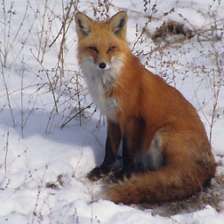
\includegraphics[width=0.085\textwidth]{figures/ptnb_v2/qualitative/butterfly/red_fox_snow/original.png}
        & 
\includegraphics[width=0.085\textwidth]{figures/ptnb_v2/qualitative/butterfly/red_fox_snow/mask.png}
        & 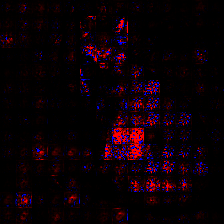
\includegraphics[width=0.085\textwidth]{figures/ptnb_v2/qualitative/butterfly/red_fox_snow/rg_loc.png}
        & 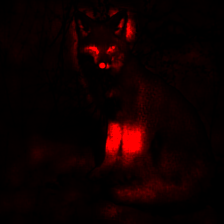
\includegraphics[width=0.085\textwidth]{figures/ptnb_v2/qualitative/butterfly/red_fox_snow/rgeq_loc.png}
        & 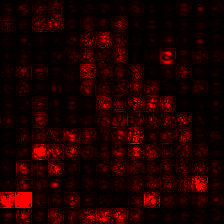
\includegraphics[width=0.085\textwidth]{figures/ptnb_v2/qualitative/butterfly/red_fox_snow/gradient.png}
        & 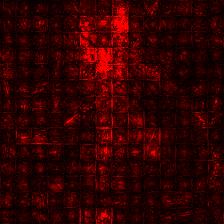
\includegraphics[width=0.085\textwidth]{figures/ptnb_v2/qualitative/butterfly/red_fox_snow/smooth_grad.png}
        & 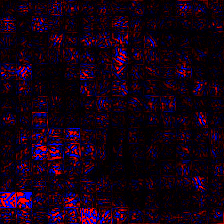
\includegraphics[width=0.085\textwidth]{figures/ptnb_v2/qualitative/butterfly/red_fox_snow/integrated_gradients.png}
        & 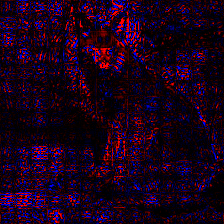
\includegraphics[width=0.085\textwidth]{figures/ptnb_v2/qualitative/butterfly/red_fox_snow/dave.png}
        & 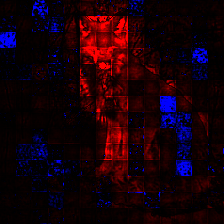
\includegraphics[width=0.085\textwidth]{figures/ptnb_v2/qualitative/butterfly/red_fox_snow/lrp_gamma.png}
        & 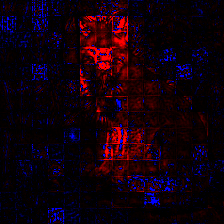
\includegraphics[width=0.085\textwidth]{figures/ptnb_v2/qualitative/butterfly/red_fox_snow/attn_lrp.png}
        & 
\includegraphics[width=0.085\textwidth]{figures/ptnb_v2/qualitative/butterfly/red_fox_snow/tibav.png} \\[1pt]
        \rotatebox{90}{\scriptsize\hspace{6pt}Red fox}
        & 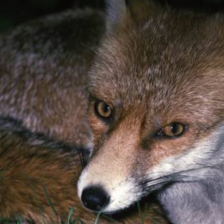
\includegraphics[width=0.085\textwidth]{figures/ptnb_v2/qualitative/butterfly/red_fox/original.png}
        & 
\includegraphics[width=0.085\textwidth]{figures/ptnb_v2/qualitative/butterfly/red_fox/mask.png}
        & 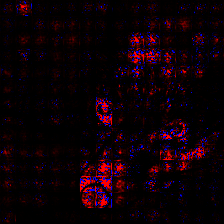
\includegraphics[width=0.085\textwidth]{figures/ptnb_v2/qualitative/butterfly/red_fox/rg_loc.png}
        & 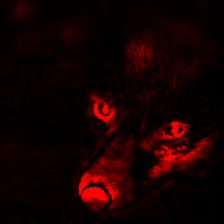
\includegraphics[width=0.085\textwidth]{figures/ptnb_v2/qualitative/butterfly/red_fox/rgeq_loc.png}
        & 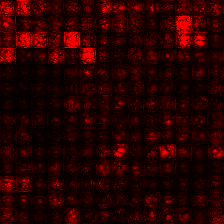
\includegraphics[width=0.085\textwidth]{figures/ptnb_v2/qualitative/butterfly/red_fox/gradient.png}
        & 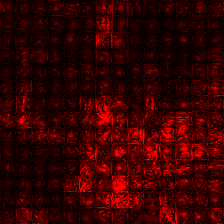
\includegraphics[width=0.085\textwidth]{figures/ptnb_v2/qualitative/butterfly/red_fox/smooth_grad.png}
        & 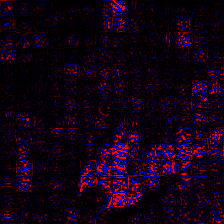
\includegraphics[width=0.085\textwidth]{figures/ptnb_v2/qualitative/butterfly/red_fox/integrated_gradients.png}
        & 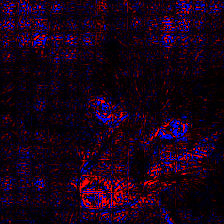
\includegraphics[width=0.085\textwidth]{figures/ptnb_v2/qualitative/butterfly/red_fox/dave.png}
        & 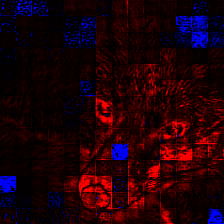
\includegraphics[width=0.085\textwidth]{figures/ptnb_v2/qualitative/butterfly/red_fox/lrp_gamma.png}
        & 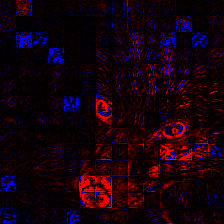
\includegraphics[width=0.085\textwidth]{figures/ptnb_v2/qualitative/butterfly/red_fox/attn_lrp.png}
        & 
\includegraphics[width=0.085\textwidth]{figures/ptnb_v2/qualitative/butterfly/red_fox/tibav.png} \\[1pt]
        \rotatebox{90}{\scriptsize\hspace{9pt}Kuvasz}
        & 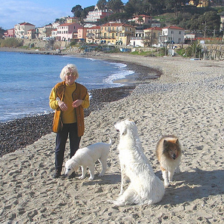
\includegraphics[width=0.085\textwidth]{figures/ptnb_v2/qualitative/butterfly/kuvasz/original.png}
        & 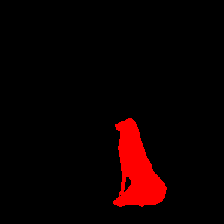
\includegraphics[width=0.085\textwidth]{figures/ptnb_v2/qualitative/butterfly/kuvasz/mask.png}
        & 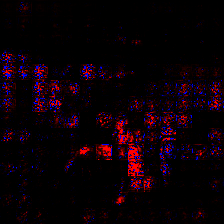
\includegraphics[width=0.085\textwidth]{figures/ptnb_v2/qualitative/butterfly/kuvasz/rg_loc.png}
        & 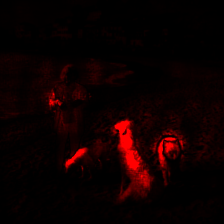
\includegraphics[width=0.085\textwidth]{figures/ptnb_v2/qualitative/butterfly/kuvasz/rgeq_loc.png}
        & 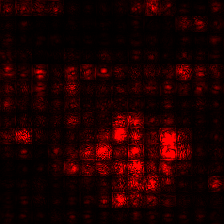
\includegraphics[width=0.085\textwidth]{figures/ptnb_v2/qualitative/butterfly/kuvasz/gradient.png}
        & 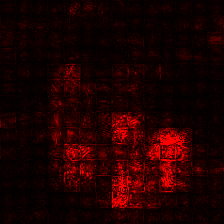
\includegraphics[width=0.085\textwidth]{figures/ptnb_v2/qualitative/butterfly/kuvasz/smooth_grad.png}
        & 
\includegraphics[width=0.085\textwidth]{figures/ptnb_v2/qualitative/butterfly/kuvasz/integrated_gradients.png}
        & 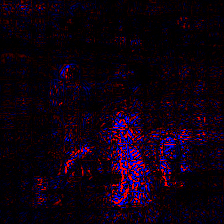
\includegraphics[width=0.085\textwidth]{figures/ptnb_v2/qualitative/butterfly/kuvasz/dave.png}
        & 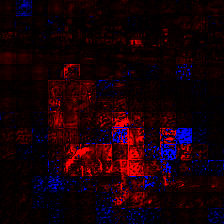
\includegraphics[width=0.085\textwidth]{figures/ptnb_v2/qualitative/butterfly/kuvasz/lrp_gamma.png}
        & 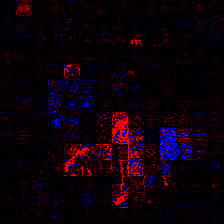
\includegraphics[width=0.085\textwidth]{figures/ptnb_v2/qualitative/butterfly/kuvasz/attn_lrp.png}
        & 
\includegraphics[width=0.085\textwidth]{figures/ptnb_v2/qualitative/butterfly/kuvasz/tibav.png} \\[1pt]
        \rotatebox{90}{\scriptsize\hspace{7pt}Wild boar}
        & 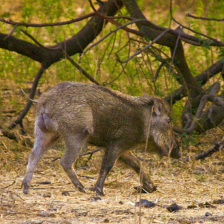
\includegraphics[width=0.085\textwidth]{figures/ptnb_v2/qualitative/butterfly/wild_boar/original.png}
        & 
\includegraphics[width=0.085\textwidth]{figures/ptnb_v2/qualitative/butterfly/wild_boar/mask.png}
        & 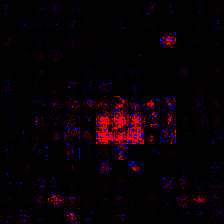
\includegraphics[width=0.085\textwidth]{figures/ptnb_v2/qualitative/butterfly/wild_boar/rg_loc.png}
        & 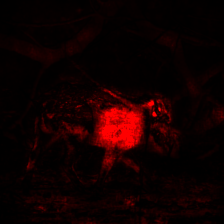
\includegraphics[width=0.085\textwidth]{figures/ptnb_v2/qualitative/butterfly/wild_boar/rgeq_loc.png}
        & 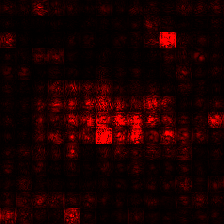
\includegraphics[width=0.085\textwidth]{figures/ptnb_v2/qualitative/butterfly/wild_boar/gradient.png}
        & 
\includegraphics[width=0.085\textwidth]{figures/ptnb_v2/qualitative/butterfly/wild_boar/smooth_grad.png}
        & 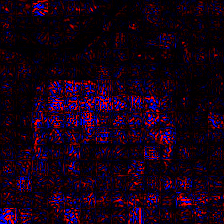
\includegraphics[width=0.085\textwidth]{figures/ptnb_v2/qualitative/butterfly/wild_boar/integrated_gradients.png}
        & 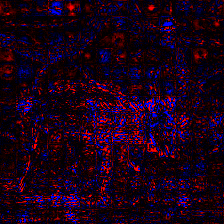
\includegraphics[width=0.085\textwidth]{figures/ptnb_v2/qualitative/butterfly/wild_boar/dave.png}
        & 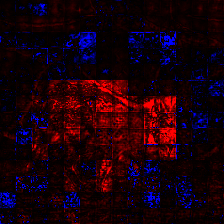
\includegraphics[width=0.085\textwidth]{figures/ptnb_v2/qualitative/butterfly/wild_boar/lrp_gamma.png}
        & 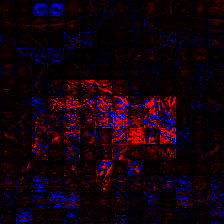
\includegraphics[width=0.085\textwidth]{figures/ptnb_v2/qualitative/butterfly/wild_boar/attn_lrp.png}
        & 
\includegraphics[width=0.085\textwidth]{figures/ptnb_v2/qualitative/butterfly/wild_boar/tibav.png} \\[1pt]
        \rotatebox{90}{\scriptsize\hspace{5pt}Black bear}
        & 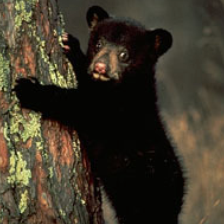
\includegraphics[width=0.085\textwidth]{figures/ptnb_v2/qualitative/butterfly/american_black_bear/original.png}
        & 
\includegraphics[width=0.085\textwidth]{figures/ptnb_v2/qualitative/butterfly/american_black_bear/mask.png}
        & 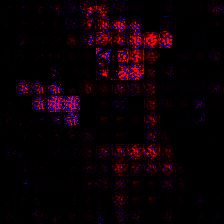
\includegraphics[width=0.085\textwidth]{figures/ptnb_v2/qualitative/butterfly/american_black_bear/rg_loc.png}
        & 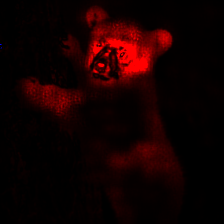
\includegraphics[width=0.085\textwidth]{figures/ptnb_v2/qualitative/butterfly/american_black_bear/rgeq_loc.png}
        & 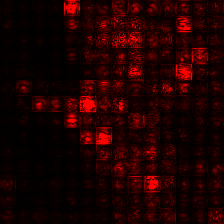
\includegraphics[width=0.085\textwidth]{figures/ptnb_v2/qualitative/butterfly/american_black_bear/gradient.png}
        & 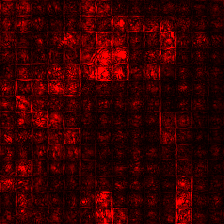
\includegraphics[width=0.085\textwidth]{figures/ptnb_v2/qualitative/butterfly/american_black_bear/smooth_grad.png}
        & 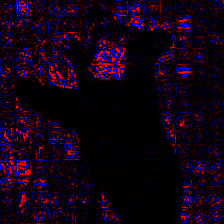
\includegraphics[width=0.085\textwidth]{figures/ptnb_v2/qualitative/butterfly/american_black_bear/integrated_gradients.png}
        & 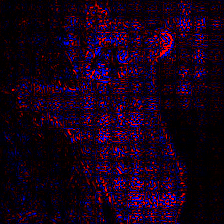
\includegraphics[width=0.085\textwidth]{figures/ptnb_v2/qualitative/butterfly/american_black_bear/dave.png}
        & 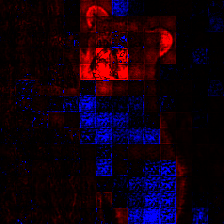
\includegraphics[width=0.085\textwidth]{figures/ptnb_v2/qualitative/butterfly/american_black_bear/lrp_gamma.png}
        & 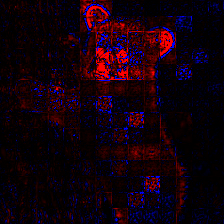
\includegraphics[width=0.085\textwidth]{figures/ptnb_v2/qualitative/butterfly/american_black_bear/attn_lrp.png}
        & 
\includegraphics[width=0.085\textwidth]{figures/ptnb_v2/qualitative/butterfly/american_black_bear/tibav.png} \\[1pt]
        \rotatebox{90}{\scriptsize\hspace{9pt}Airliner}
        & 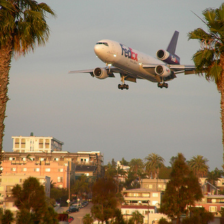
\includegraphics[width=0.085\textwidth]{figures/ptnb_v2/qualitative/butterfly/airliner/original.png}
        & 
\includegraphics[width=0.085\textwidth]{figures/ptnb_v2/qualitative/butterfly/airliner/mask.png}
        & 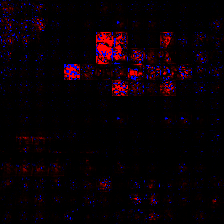
\includegraphics[width=0.085\textwidth]{figures/ptnb_v2/qualitative/butterfly/airliner/rg_loc.png}
        & 
\includegraphics[width=0.085\textwidth]{figures/ptnb_v2/qualitative/butterfly/airliner/rgeq_loc.png}
        & 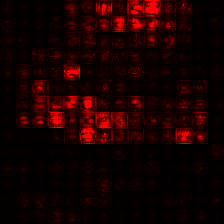
\includegraphics[width=0.085\textwidth]{figures/ptnb_v2/qualitative/butterfly/airliner/gradient.png}
        & 
\includegraphics[width=0.085\textwidth]{figures/ptnb_v2/qualitative/butterfly/airliner/smooth_grad.png}
        & 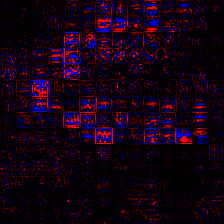
\includegraphics[width=0.085\textwidth]{figures/ptnb_v2/qualitative/butterfly/airliner/integrated_gradients.png}
        & 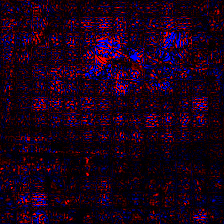
\includegraphics[width=0.085\textwidth]{figures/ptnb_v2/qualitative/butterfly/airliner/dave.png}
        & 
\includegraphics[width=0.085\textwidth]{figures/ptnb_v2/qualitative/butterfly/airliner/lrp_gamma.png}
        & 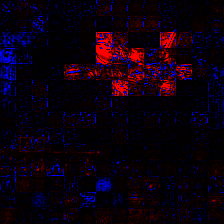
\includegraphics[width=0.085\textwidth]{figures/ptnb_v2/qualitative/butterfly/airliner/attn_lrp.png}
        & 
\includegraphics[width=0.085\textwidth]{figures/ptnb_v2/qualitative/butterfly/airliner/tibav.png} \\
    \end{tabular}
    }
    }%
\caption[ViT-B/16 qualitative comparison on six ImageNet-S examples]{Six ImageNet-S examples, ViT-B/16, at the configurations specified above. Red and blue show positive and negative attribution. Each sign is divided by its image-wide 99th percentile and clipped, saturating the top 1\% so concentrated maps remain legible; every method uses this display transform.}
    \label{ptnb:fig:qualitative}
\end{figure}
\par\medskip


\chapter{Publication Provenance and Tool Use}\label{app:publication_provenance}

This thesis integrates two coauthored works with the thesis author as first author: \emph{Hidden Monotonicity}, a CVPR 2026 Highlight~\parencite{hiddenMono}, and the revised \emph{Playing the Network Backward} preprint, arXiv:2605.06212v2~\parencite{playingBackward2026}, without a claim of AISTATS acceptance. It reuses their model-evaluation outputs and point estimates, recomputing VOC intervals and paired comparisons by whole-image resampling (Section~\ref{ptnb:app:stats}). A shared decomposition framework adds common definitions, mathematical extensions, connections and Lean formalization.

\section{Author's Contribution}\label{app:author_contribution}

For both papers, I developed the theory and experiments, ran the experiments, and wrote all appendices and most text outside the introductions, collaborating with the coauthors listed in Section~\ref{sec:motivation}.

The following disclosures distinguish original-paper preparation from later thesis work.

\section{Disclosure in the Revised Game Paper}
The revised game paper discloses the following for its preparation:
\begin{quote}
In this work, we used generative AI tools for implementing standard baseline methods and evaluation
code, for producing plots and tables of results, for drafting parts of the text, and for editing
(grammar, spelling, word choice, and reformatting).
We have not used generative AI tools to generate research ideas, to formulate the games, or to
produce the theorems and their proofs.
All AI-assisted code was reviewed and tested by the authors, including unit tests that check the
game-theoretic occupation measures against reference gradient and $\alpha\beta$-LRP
implementations; all AI-assisted text was checked by the authors for correctness, and every
reference was verified manually.
We take responsibility for the final content of this work, including text, claims, and artifacts
produced with the aid of generative AI.
\end{quote}

\section{AI Assistance in the Thesis Revision}
The November 2026 thesis revision used OpenAI's Codex for mathematical exploration, proof development, Lean implementation and checking, code review and repair, statistical reaggregation, and drafting and editing. Mathematical assistance developed and checked convex, monotone stream extensions. The quoted historical statement about theorem and proof development concerns the original paper, excluding this later thesis work.

The formalization repository records reviewed theorem types, proof-checking receipts and coverage limits. Lean certifies the stated propositions; source correspondence requires mathematical review, and kernel checks do not certify experiments.
